\documentclass[journal,compsoc]{IEEEtran}
%DIF LATEXDIFF DIFFERENCE FILE
%DIF DEL ./original-export/main.tex   Thu Oct 29 14:07:26 2015
%DIF ADD ./main.tex                   Thu Oct 29 15:10:01 2015
\pagenumbering{arabic}

\usepackage{booktabs}
\usepackage{multirow}
%\usepackage{graphix}
\usepackage{lscape}

\usepackage{amssymb}
\usepackage{amsmath}
\usepackage{balance}  % to better equalize the last page
\usepackage{graphicx} % for EPS, load graphicx instead
\usepackage{times}    % comment if you want LaTeX's default font
\usepackage{url}      % llt: nicely formatted URLs
\usepackage[lofdepth,lotdepth]{subfig}
%\usepackage[pdftex]{hyperref}
\usepackage{multirow}
\usepackage{bbm}
\usepackage{pseudocode}
\usepackage{color}
%DIF 21c21
%DIF < %\usepackage{cite}
%DIF -------
\usepackage{cite} %DIF > 
%DIF -------
%\usepackage{algorithmic}
%\usepackage{algorithm}
%\usepackage[noend]{algpseudocode}
%\usepackage{algorithm}
\usepackage{algpseudocode}
\usepackage[linesnumbered,boxed,ruled]{algorithm2e}

%\newcommand{\modf3}[1]{\textcolor{blue}{#1}}

\newcommand{\TheName}{\mbox{\emph{Daehr}}}
\newcommand{\modif}[1]{\textcolor{blue}{#1}}
%DIF PREAMBLE EXTENSION ADDED BY LATEXDIFF
%DIF UNDERLINE PREAMBLE %DIF PREAMBLE
\RequirePackage[normalem]{ulem} %DIF PREAMBLE
\RequirePackage{color}\definecolor{RED}{rgb}{1,0,0}\definecolor{BLUE}{rgb}{0,0,1} %DIF PREAMBLE
\providecommand{\DIFadd}[1]{{\protect\color{blue}\uwave{#1}}} %DIF PREAMBLE
\providecommand{\DIFdel}[1]{{\protect\color{red}\sout{#1}}}                      %DIF PREAMBLE
%DIF SAFE PREAMBLE %DIF PREAMBLE
\providecommand{\DIFaddbegin}{} %DIF PREAMBLE
\providecommand{\DIFaddend}{} %DIF PREAMBLE
\providecommand{\DIFdelbegin}{} %DIF PREAMBLE
\providecommand{\DIFdelend}{} %DIF PREAMBLE
%DIF FLOATSAFE PREAMBLE %DIF PREAMBLE
\providecommand{\DIFaddFL}[1]{\DIFadd{#1}} %DIF PREAMBLE
\providecommand{\DIFdelFL}[1]{\DIFdel{#1}} %DIF PREAMBLE
\providecommand{\DIFaddbeginFL}{} %DIF PREAMBLE
\providecommand{\DIFaddendFL}{} %DIF PREAMBLE
\providecommand{\DIFdelbeginFL}{} %DIF PREAMBLE
\providecommand{\DIFdelendFL}{} %DIF PREAMBLE
%DIF END PREAMBLE EXTENSION ADDED BY LATEXDIFF

\begin{document}
\title{\TheName{}: a Linear Discriminant Analysis Framework for Electronic Health Record Data \\
 {\LARGE with its Application to Early Detection of Mental Health Disorders}}

\author{\IEEEauthorblockN{Haoyi Xiong,~Jinghe Zhang,~Yu Huang,~Kevin Leach, and ~Laura E. Barnes}~\DIFdelbegin %DIFDELCMD < \thanks{Authors are all with Department of Systems and Information Engineering, University of Virginia, VA. Email:\{hx6d, xxx, xxx, xxx\}@virginian.edu}
%DIFDELCMD < %%%
\DIFdelend \DIFaddbegin \thanks{Authors are all with Department of Systems and Information Engineering, University of Virginia, VA. Email:\{hx6d, xxx, xxx, xxx\}@virginia.edu}
\DIFaddend }

\DIFdelbegin %DIFDELCMD < \IEEEcompsoctitleabstractindextext{
%DIFDELCMD < \begin{abstract}
%DIFDELCMD < 

%DIFDELCMD < Electronic Health Records (EHR), consisting of massive patients'  diagnosis records, have been used to predict patients' future or potential diseases according to their past diagnoses.
%DIFDELCMD < While tons of data mining tools have been adopted for EHR-based disease early detection, Linear Discriminant Analysis (LDA) is one of the most commonly used statistical methods.
%DIFDELCMD < However, it is hard to train an accurate LDA model to early detect specific diseases when the known patients with the targeted diseases are few and the EHR data are coded manually with noise, since in such case the covariance matrices used in LDA are usually singular and estimated with large variance.
%DIFDELCMD < With above issues in mind, this paper presents \TheName\ -- an extending LDA framework using Electronic Health Records.
%DIFDELCMD < Beyond the existing LDA analyzers, \TheName\ is proposed to 1) eliminate the data noise caused by the manual encoding of EHR data, and 2) lower the variance of LDA model even when only a few patients' EHR are given for training.
%DIFDELCMD < To achieve the two goals, we designed an iterative algorithm to improve the covariance matrix estimation with embedded data noise/variance reduction for LDA.
%DIFDELCMD < We evaluated \TheName\ extensively using a large-scale real-world EHR dataset -- CHSN.
%DIFDELCMD < Specifically, our experiments compared the performance of LDA to the three baselines (i.e., LDA and its derivatives),  in terms of identifying high risk college students potentially with mental health disorders from 23 US universities.
%DIFDELCMD < Experiment results showed \TheName\ significantly outperformed three baselines by achieving 3\%--10\% higher prediction accuracy, and 3\% --14\% higher F1-score.
%DIFDELCMD < 

%DIFDELCMD < \end{abstract}
%DIFDELCMD < 

%DIFDELCMD < \begin{IEEEkeywords}
%DIFDELCMD < predictive models, early detection, anxiety/depression, temporal order, electronic health data
%DIFDELCMD < \end{IEEEkeywords}
%DIFDELCMD < }
%DIFDELCMD < %%%
\DIFdelend \DIFaddbegin \IEEEcompsoctitleabstractindextext{ \begin{abstract} Electronic Health Records (EHR) containing a massive number of patients' diagnosis records have been used to predict future or potential diseases according to their past diagnoses.
While a number of data mining tools have been adopted for EHR-based early disease detection, Linear Discriminant Analysis (LDA) is one of the most commonly used statistical methods.
However, it is difficult to train an accurate LDA model that detects specific diseases when there are too few known patients with the targeted diseases and the EHR data are coded manually with noise, because the covariance matrices used in LDA are usually singular and estimated with large variance.
To address these issues, this paper presents \TheName{}, an extended LDA framework using Electronic Health Records.
Beyond the existing LDA analyzers, \TheName{} is proposed to 1) eliminate the data noise caused by the manual encoding of EHR data, and 2) lower the variance of the LDA model even when only a few patients' EHR data are given for training.
To achieve the two goals, we designed an iterative algorithm to improve the covariance matrix estimation with embedded data noise/variance reduction for LDA.
We evaluated \TheName{} extensively using a large-scale real-world EHR dataset, the College Health Surveillance Network (CHSN).
Specifically, our experiments compare the performance of LDA to three baselines (i.e., LDA and its derivatives) in terms of identifying high risk college students for mental health disorders from 23 US universities.
Experimental results show that \TheName{} significantly outperformed three baselines by achieving 3\%--10\% higher prediction accuracy, and a 3\% --14\% higher F1-score.


\end{abstract}

\begin{IEEEkeywords}
predictive models, early detection, anxiety/depression, temporal order, electronic health data
\end{IEEEkeywords}
}
\DIFaddend \maketitle
\IEEEpeerreviewmaketitle

% For peer review papers, you can put extra information on the cover
% page as needed:
% \ifCLASSOPTIONpeerreview
% \begin{center} \bfseries EDICS Category: 3-BBND \end{center}
% \fi
%
% For peerreview papers, this IEEEtran command inserts a page break and
% creates the second title. It will be ignored for other modes.
\IEEEpeerreviewmaketitle

\section{Introduction}

With the rapid development of medical big data, forecasting future or potential \DIFdelbegin \DIFdel{disease }\DIFdelend \DIFaddbegin \DIFadd{diseases }\DIFaddend based on patients' past medical records \DIFdelbegin \DIFdel{becomes a promising way to detect and further prevent high risk disease in advance.
Instead of paying attentions }\DIFdelend \DIFaddbegin \DIFadd{has emerged as a promising approach towards preventing high-risk diseases.
Rather than individualizing patients }\DIFaddend (e.g., \DIFaddbegin \DIFadd{via }\DIFaddend screening or counseling)\DIFdelbegin \DIFdel{to all its patient intensively}\DIFdelend , a medical \DIFaddbegin \DIFadd{informatics }\DIFaddend system can predict each patient's potential diseases using his \DIFdelbegin \DIFdel{/}\DIFdelend \DIFaddbegin \DIFadd{or }\DIFaddend her past diagnoses as well as \DIFdelbegin \DIFdel{the diagnoses records collected from massive }\DIFdelend \DIFaddbegin \DIFadd{diagnoses collected from many }\DIFaddend other patients.
In this way, the medical system can identify \DIFdelbegin \DIFdel{high risk patients from the all }\DIFdelend \DIFaddbegin \DIFadd{high-risk patients from a large corpus of }\DIFaddend patients with low cost\DIFdelbegin \DIFdel{, then serve patients in a targeted manner, further start prevention }\DIFdelend \DIFaddbegin \DIFadd{.
These high-risk patients can then receive targeted care to employ disease prevention techniques }\DIFaddend in advance.
\DIFdelbegin \DIFdel{Therefore}\DIFdelend \DIFaddbegin \DIFadd{Naturally}\DIFaddend , the accuracy of \DIFdelbegin \DIFdel{disease early detection is a crucial factor to improve }\DIFdelend \DIFaddbegin \DIFadd{such early disease detection is crucial to improving }\DIFaddend the efficiency of \DIFdelbegin \DIFdel{high risk }\DIFdelend \DIFaddbegin \DIFadd{high-risk }\DIFaddend patient identification and disease prevention. 


In this paper\DIFdelbegin \DIFdel{we present \TheName}\DIFdelend \DIFaddbegin \DIFadd{, we present \TheName{}}\DIFaddend ---an \DIFdelbegin \DIFdel{extending }\DIFdelend \DIFaddbegin \DIFadd{extended }\DIFaddend linear discriminant analysis (LDA)~\cite{fisher1936use,mclachlan2004discriminant} framework for \DIFdelbegin \DIFdel{disease early }\DIFdelend \DIFaddbegin \DIFadd{early disease }\DIFaddend detection using Electronic Health Records (EHR), which can improve the prediction accuracy of the standard LDA model \DIFdelbegin \DIFdel{through reducing the }\DIFdelend \DIFaddbegin \DIFadd{by reducing }\DIFaddend noise in EHR data and regularizing the estimated covariance matrices.
\DIFdelbegin \DIFdel{In the rest of this section, we }\DIFdelend \DIFaddbegin \DIFadd{We }\DIFaddend first discuss the motivations and background of this research, then we formulate a new research problem based on our observations and assumptions.
We elaborate the technical challenges of the proposed research\DIFdelbegin \DIFdel{and finally }\DIFdelend \DIFaddbegin \DIFadd{. 
Finally, }\DIFaddend we summarize our technical contributions.


\subsection{Motivations and Backgrounds}

\DIFdelbegin \DIFdel{In order to }\DIFdelend \DIFaddbegin \DIFadd{To }\DIFaddend predict patients' potential \DIFdelbegin \DIFdel{disease }\DIFdelend \DIFaddbegin \DIFadd{diseases }\DIFaddend according to their past medical records, a variety of predictive models utilizing heterogeneous medical data have been studied~\cite{soni2011predictive,palaniappan2008intelligent,kumari2011comparative}\DIFdelbegin \DIFdel{, such as chest imaging for chest cancer early detection }\DIFdelend \DIFaddbegin \DIFadd{.
For example, chest imaging has been used for early detection of chest cancer~\mbox{%DIFAUXCMD
\cite{FIXME}
}%DIFAUXCMD
}\DIFaddend , questionnaire-based assessment (e.g., PHQ-9~\cite{kroenke2002phq}) data for \DIFdelbegin \DIFdel{mental disorder prediction}\DIFdelend \DIFaddbegin \DIFadd{predicting mental disorders}\DIFaddend , and screening data for \DIFdelbegin \DIFdel{heart disease prediction}\DIFdelend \DIFaddbegin \DIFadd{predicting heart disease}\DIFaddend ~\cite{d2001validation}.
Among \DIFdelbegin \DIFdel{all }\DIFdelend these medical data, Electronic Health Records (EHR) consisting of the diagnosis records \DIFdelbegin \DIFdel{of patients' each visit }\DIFdelend \DIFaddbegin \DIFadd{from patients' visits }\DIFaddend are used as a general purpose data source that enables \DIFdelbegin \DIFdel{massive disease early }\DIFdelend \DIFaddbegin \DIFadd{early disease }\DIFaddend detection based on the previous diagnoses \DIFaddbegin \DIFadd{at a massive scale}\DIFaddend .
Furthermore, this data \DIFdelbegin \DIFdel{has a higher accessibility }\DIFdelend \DIFaddbegin \DIFadd{is more accessible }\DIFaddend to clinicians and researchers\DIFaddbegin \DIFadd{, }\DIFaddend and holds comprehensive information of patients\DIFdelbegin \DIFdel{medical history }\DIFdelend \DIFaddbegin \DIFadd{' medical history, }\DIFaddend especially within the primary care setting.
Thus, EHR data \DIFdelbegin \DIFdel{also }\DIFdelend provides a promising opportunity for \DIFdelbegin \DIFdel{the disease early }\DIFdelend \DIFaddbegin \DIFadd{early disease }\DIFaddend detection due to its \DIFdelbegin \DIFdel{general-purposeness, accessibility}\DIFdelend \DIFaddbegin \DIFadd{generality, accessibility, }\DIFaddend and standardized use and features. 


As shown in \DIFdelbegin \DIFdel{Fig}\DIFdelend \DIFaddbegin \DIFadd{Figure}\DIFaddend ~\ref{fig:exp-ehr}, a patient's EHR data includes all his/her past diagnosis and treatment records, where the diagnosis record includes a sequence of visits\DIFdelbegin \DIFdel{and each visits }\DIFdelend \DIFaddbegin \DIFadd{, and each visit }\DIFaddend consists of multiple diagnoses.
\DIFdelbegin \DIFdel{Please note }\DIFdelend \DIFaddbegin \DIFadd{Note }\DIFaddend that all diagnoses are recorded using ICD-9 codes~\cite{dubberke2006icd}, where each evidence of diagnosis corresponds to a specific ICD-9 code.
With diagnosis records in the EHR data, several methods~\cite{personalized2015, amarasingham2010automated, pittman2004integrated,jensen2012mining} have been studied to predict the disease of patients.
Given a disease as the prediction target (e.g., anxiety/depression) as well as the EHR data of a large population with \DIFdelbegin \DIFdel{/out }\DIFdelend \DIFaddbegin \DIFadd{or without }\DIFaddend the target disease, most \DIFdelbegin \DIFdel{of }\DIFdelend existing methods first represent each given patient's EHR data using a set of features, and then train a predictive model using features and labels (if each patient is diagnosed with the targeted disease) in a supervised manner.
Further, given each new patient's EHR data, these models predict if the given patient will develop the targeted disease in near future using the trained predictive model.


\begin{figure}
\centering
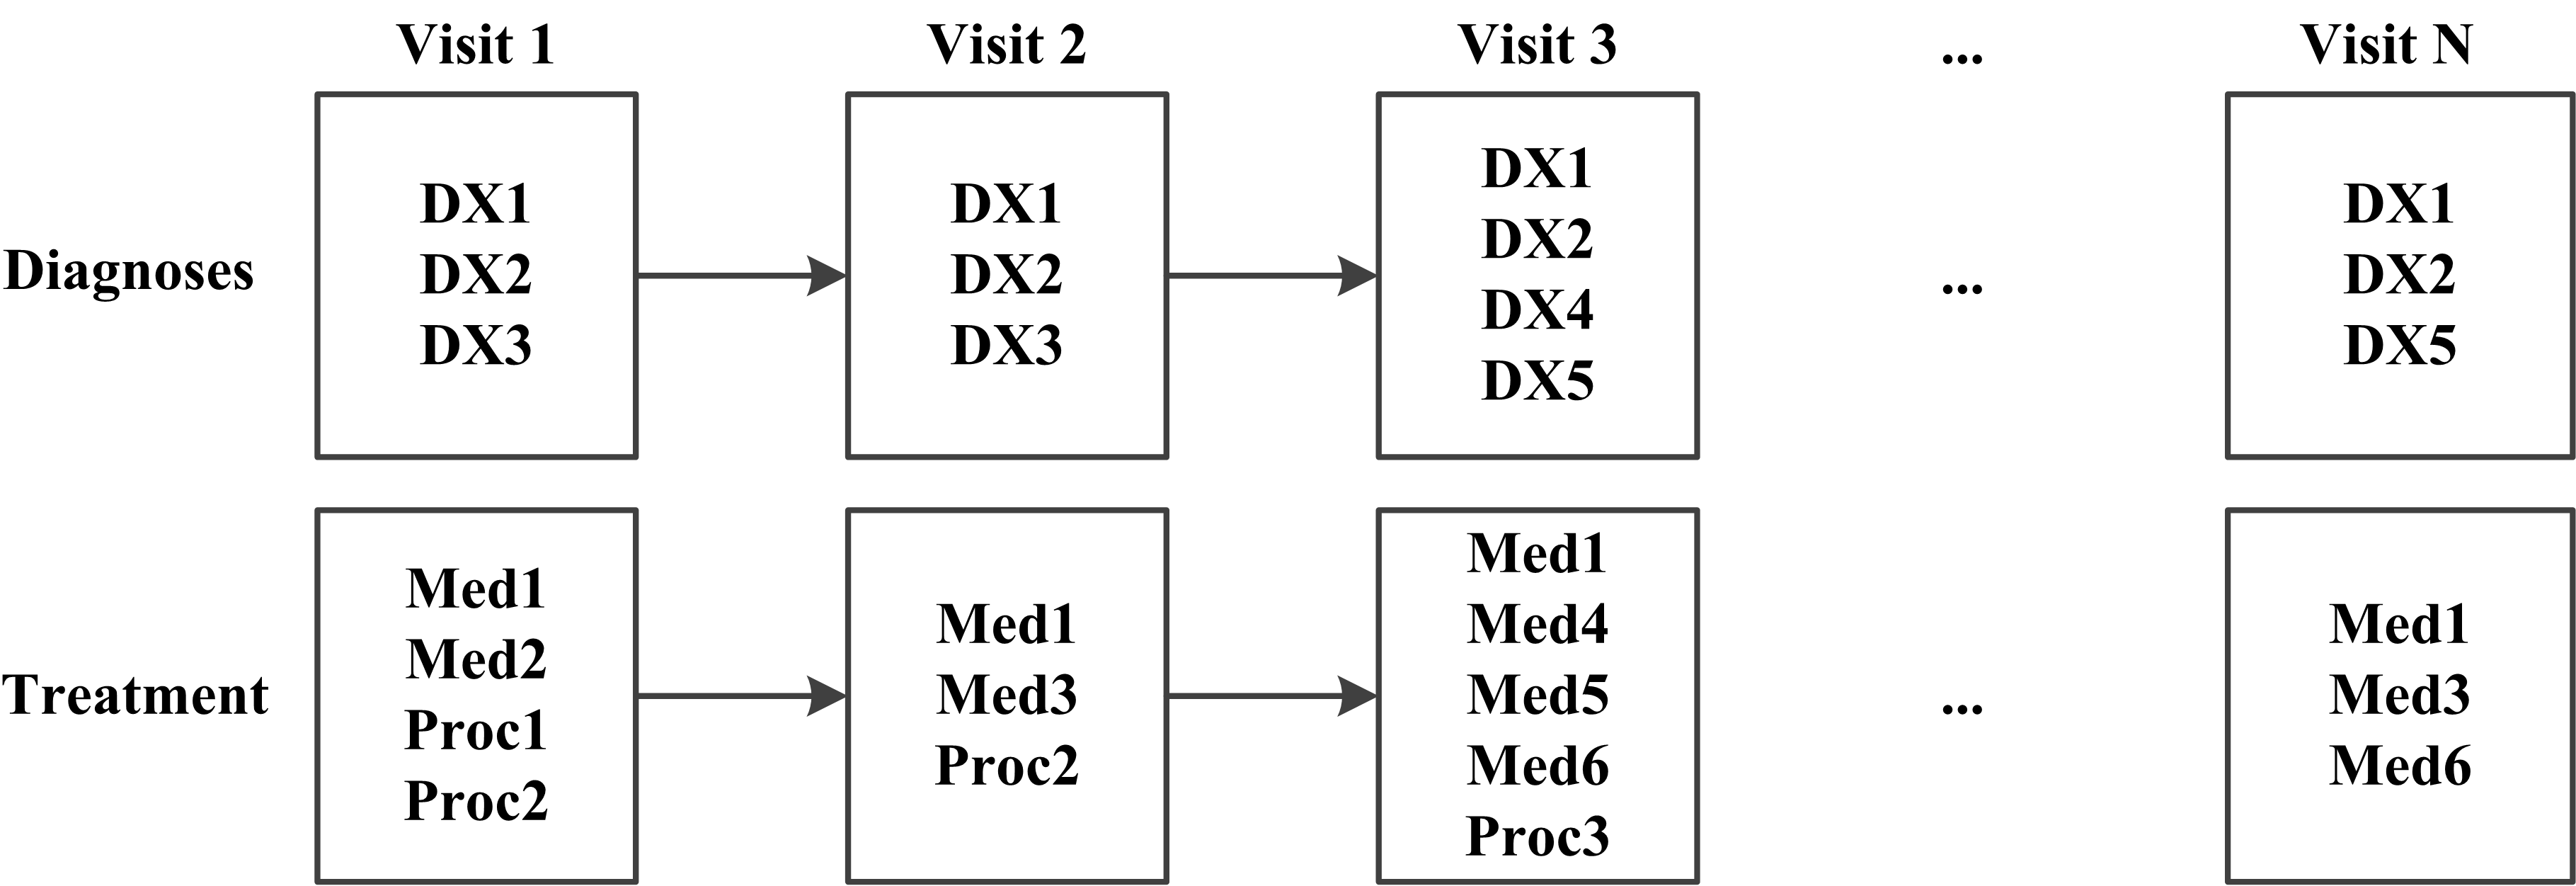
\includegraphics[width=0.48\textwidth]{./img/Patient.png}
\caption{An Example of a Patient's EHR Data}
\label{fig:exp-ehr}
\end{figure}


\textbf{EHR Data Representation for Early Detection.} 
In terms of representing EHR data, existing approaches include using diagnosis-frequencies~\cite{sun2012supervised,7091853,personalized2015}, pairwise diagnosis transitions~\cite{zhang_mseq_2015,jensen2001mining}, graph representations of diagnosis sequences~\cite{liu_temporal_2015}, and so on.
Among these approaches, the diagnosis-frequency is \DIFdelbegin \DIFdel{considered as one of common ways }\DIFdelend \DIFaddbegin \DIFadd{one common way }\DIFaddend to represent EHR data.
Given each patient's EHR data, which consists of the patient's demographic information and a sequence of past visits, existing methods first retrieve the diagnosis codes recorded during each visit.
\DIFdelbegin \DIFdel{Then}\DIFdelend \DIFaddbegin \DIFadd{Next}\DIFaddend , the frequency of each diagnosis appearing in all past visits are counted, followed by further transformation on the frequency of each diagnosis into a vector of frequencies (e.g., $\langle 1, 0, \dots, 3\rangle$, where 0 means the \DIFdelbegin \DIFdel{$2^{nd}$ diagnoses }\DIFdelend \DIFaddbegin \DIFadd{second diagnosis }\DIFaddend does not exist in all past visits).
In this way, each patient having different number of visits and each visit consisting of multiple diagnoses is represented as a fixed-length data vector, which can be handled by common machine learning algorithms.


\DIFdelbegin \DIFdel{Please note }\DIFdelend \DIFaddbegin \DIFadd{Note }\DIFaddend that the diagnosis-frequency representation of EHR data is usually with ultra-high dimensions; for example, there \DIFdelbegin \DIFdel{exists }\DIFdelend \DIFaddbegin \DIFadd{are }\DIFaddend more than 15,000 ICD-9 codes in \DIFaddbegin \DIFadd{the }\DIFaddend EHR scheme, thus the diagnosis-frequency vector using raw ICD-9 codes \DIFdelbegin \DIFdel{is usually with }\DIFdelend \DIFaddbegin \DIFadd{contains }\DIFaddend thousands of dimensions.
\DIFdelbegin \DIFdel{In order to reduce the dimensinality}\DIFdelend \DIFaddbegin \DIFadd{To reduce the dimensionality}\DIFaddend , clinical professionals may suggest \DIFdelbegin \DIFdel{to use clustered code set}\DIFdelend \DIFaddbegin \DIFadd{using clustered code sets}\DIFaddend , where each ICD-9 code can map to one of the 295 clustered codes.
\DIFdelbegin \DIFdel{In this way}\DIFdelend \DIFaddbegin \DIFadd{Thus}\DIFaddend , each raw diagnosis-frequency vector can be compressed to a vector of around 200 dimensions using clustered codes.


\textbf{Supervised Learning for Early Detection.} 
Given an EHR database and a target disease for early detection, existing \DIFdelbegin \DIFdel{method usually needs to }\DIFdelend \DIFaddbegin \DIFadd{methods }\DIFaddend first select patients both with and without the disease, then use \DIFaddbegin \DIFadd{an appropriate representation of }\DIFaddend their EHR data \DIFdelbegin \DIFdel{with appropriate representation }\DIFdelend to form a training set.
\DIFdelbegin \DIFdel{In order to }\DIFdelend \DIFaddbegin \DIFadd{To }\DIFaddend train an accurate predictive model with the training set, \DIFdelbegin \DIFdel{a lot of }\DIFdelend \DIFaddbegin \DIFadd{many }\DIFaddend machine learning methods such as Support Vector Machine (SVM), Random Forest (RF), Bayesian Network, Gaussian Process and Linear Discriminant Analysis (LDA) have been adopted~\cite{sun2012supervised,7091853,personalized2015,zhang_mseq_2015,jensen2001mining,liu_temporal_2015,cazzanti_local_2007}.
Among these machine learning methods, LDA is frequently used as one of the common performance benchmarks in a series of studies~\cite{cazzanti_local_2007,zhang_mseq_2015,kalina2013selecting,karlsson2014handling,wang2014clinical} \DIFdelbegin \DIFdel{, considering its capacity of dimension reduction}\DIFdelend \DIFaddbegin \DIFadd{because it effectively reduces dimensionality}\DIFaddend .
For example, when using diagnosis-frequency vector as the representation of EHR data, a LDA model learns a linear combination of diagnoses (from the all diagnoses) that can optimally separate patients into the two groups (i.e., with/without the disease).
Then\DIFdelbegin \DIFdel{LDA predicts if }\DIFdelend \DIFaddbegin \DIFadd{, LDA predicts whether }\DIFaddend new patients will develop \DIFdelbegin \DIFdel{to }\DIFdelend the targeted disease \DIFdelbegin \DIFdel{through }\DIFdelend \DIFaddbegin \DIFadd{by }\DIFaddend separating their vectors into the two groups using the linear combination.


\DIFdelbegin \DIFdel{Please be advised that, just like }\DIFdelend \DIFaddbegin \DIFadd{Like }\DIFaddend many other statistical learning models, the accuracy of a LDA model can be improved \DIFdelbegin \DIFdel{, }\DIFdelend when more samples are given for training.
\DIFdelbegin \DIFdel{It }\DIFdelend \DIFaddbegin \DIFadd{This }\DIFaddend is because the decision risk of a LDA model is inherited from the variance of its training samples, while \emph{increasing the sample size \DIFdelbegin \DIFdel{lower }\DIFdelend \DIFaddbegin \DIFadd{lowers }\DIFaddend the sample variance}~\cite{hsu1947complete,qiao2008effective}.
In contrast, when \DIFdelbegin \DIFdel{the training samples are few }\DIFdelend \DIFaddbegin \DIFadd{there are few training samples}\DIFaddend , the model \DIFdelbegin \DIFdel{even }\DIFdelend cannot produce any valid prediction results \DIFdelbegin \DIFdel{.
Because }\DIFdelend \DIFaddbegin \DIFadd{because }\DIFaddend LDA needs to use the \emph{inverse of the covariance matrices} to \DIFdelbegin \DIFdel{predict, while in such case }\DIFdelend \DIFaddbegin \DIFadd{make predictions.
In such cases, }\DIFaddend the covariance matrices estimated in LDA are singular \DIFdelbegin \DIFdel{or namely }\emph{\DIFdel{non-inversiable}} %DIFAUXCMD
\DIFdel{(i.e., the inverse of the covariance matrix doesn't exist}\DIFdelend \DIFaddbegin \DIFadd{(non-invertible}\DIFaddend )~\cite{huang2002solving,gao2006direct}.
%DIF >  KJL If the reader doesn't know what a non-invertible matrix is, there are bigger problems


\DIFdelbegin \DIFdel{With above backgrounds in mind, we }\DIFdelend \DIFaddbegin \DIFadd{We }\DIFaddend are motivated to enhance the supervised learning methods \DIFdelbegin \DIFdel{on top of EHR data , }\DIFdelend \DIFaddbegin \DIFadd{building upon EHR data }\DIFaddend so as to improve the prediction accuracy for \DIFdelbegin \DIFdel{disease early }\DIFdelend \DIFaddbegin \DIFadd{early disease }\DIFaddend detection.
Specifically, we \DIFdelbegin \DIFdel{attempts at studying }\DIFdelend \DIFaddbegin \DIFadd{study }\DIFaddend the LDA model using the diagnosis-frequency features \DIFdelbegin \DIFdel{, considering }\DIFdelend \DIFaddbegin \DIFadd{because of }\DIFaddend the relevance of such settings in clinical practices.


\subsection{Research Assumptions and Objectives}

Our research is based on following two observations and two assumptions about EHR data and early detection settings:

\textbf{Observation 1. EHR Encoding Variation \DIFdelbegin \DIFdel{- }\DIFdelend \DIFaddbegin \DIFadd{--- }\DIFaddend } 
In terms of \DIFdelbegin \DIFdel{EHR data encoding}\DIFdelend \DIFaddbegin \DIFadd{encoding EHR data}\DIFaddend , the diagnosis records are usually inputted manually by clinicians without a unified encoding scheme.
Our previous work~\DIFdelbegin \DIFdel{\mbox{%DIFAUXCMD
\cite{xxx}
}%DIFAUXCMD
}\DIFdelend \DIFaddbegin \DIFadd{\mbox{%DIFAUXCMD
\cite{FIXME}
}%DIFAUXCMD
}\DIFaddend finds that, for \DIFdelbegin \DIFdel{one patient, the }\DIFdelend \DIFaddbegin \DIFadd{a single patient, there may be a higher number of }\DIFaddend diagnosis records for one disease \DIFdelbegin \DIFdel{might be more frequent than the times that the disease has }\DIFdelend \DIFaddbegin \DIFadd{than the number of times that that disease as }\DIFaddend been diagnosed.
For example, \DIFdelbegin \emph{\DIFdel{three clinicians--Ann, Bob and Carl are working in the same clinics.
Given a patient has been diagnosed with upper respiratory infection (ICD-9 code: 465.9), Ann may only leave the record  of code 465.9 in the first visit when the disease is diagnosed.
However Bob may leave the record in the first visit as well as all his/her returning visits to receive screening/treatment for upper respiratory infection; while Carl may leave in the first visit and some of the returning visits that he feels necessary.}}  
%DIFAUXCMD
\DIFdelend \DIFaddbegin \DIFadd{consider three clinicians: Ann, Bob, and Carl, all working in the same clinic.
A single patient has been diagnosed with upper respiratory infection (ICD-9 code: 465.9).  
Ann may leave only the record of code 465.9 for the first visit in which the disease is diagnosed.
However, Bob may leave the record in the first visit as well as all of the patient's returning visits to receive screening or treatment for upper respiratory infection.
Carl may leave a record in the first visit and in some of the returning visits at his discretion.
}\DIFaddend 

\DIFdelbegin \textbf{%DIFDELCMD < \em %%%
\DIFdel{Assumption I. Non-negative Noise in Diagnosis-Frequency Vector Data - }} 
%DIFAUXCMD
\DIFdel{With the first observation in mind, it is reasonable to }\DIFdelend \DIFaddbegin \textbf{\em \DIFadd{Assumption I. Non-negative Noise in Diagnosis-Frequency Vector Data --- }} 
\DIFadd{Based upon the first observation, we }\DIFaddend assume that each diagnosis is recorded at least one time in \DIFdelbegin \DIFdel{EHR and }\DIFdelend \DIFaddbegin \DIFadd{the EHR, and that }\DIFaddend the number of records might \DIFdelbegin \DIFdel{be differing from encoding clinicians }\DIFdelend \DIFaddbegin \DIFadd{differ due to clinician encoding styles }\DIFaddend (i.e., \emph{frequency of record $\geq$ frequency of diagnosis} for each specific disease).
\DIFdelbegin \DIFdel{In this case, we }\DIFdelend \DIFaddbegin \DIFadd{We }\DIFaddend further assume the encoding variation of EHR data may cause certain unknown \emph{non-negative data noise} \DIFdelbegin \DIFdel{on top of }\DIFdelend \DIFaddbegin \DIFadd{in }\DIFaddend the diagnosis-frequency vectors.


\textbf{Observation 2. Limited Positive Training Samples \DIFdelbegin \DIFdel{- }\DIFdelend \DIFaddbegin \DIFadd{--- }\DIFaddend } 
We find that the total number of patients with a specific disease \DIFdelbegin \DIFdel{or namely }\DIFdelend \DIFaddbegin \DIFadd{(}\DIFaddend \emph{positive samples}\DIFdelbegin \DIFdel{might be so }\DIFdelend \DIFaddbegin \DIFadd{) might be too }\DIFaddend few to train a predictive model for early detection of the disease.
For example, \DIFdelbegin \emph{\DIFdel{a historically black college wants to identify the risk students in terms of mental health disorder using all students' EHR installed in the college clinics.
The clinics first sorts all students to two groups (i.e., with/without mental disorder diagnosed), then from each group it selects a subset of students as training samples.
However, due to the low utilization rate of psyclinics by African American, the available training samples with at least one type of mental disorders (e.g., depression, anxiety, mood and personality disorders) are so few (e.g., 100$-$500 students) in their school.}}  
%DIFAUXCMD
\DIFdelend \DIFaddbegin \DIFadd{consider a historically black college that wants to identify the at-risk students in terms of mental health disorders using all students' EHR data in the college clinics.
The clinics first separate all students in to two groups (i.e., with/without mental disorder diagnosed).  Then, it selects a subset of students from each group as training samples.
However, psychiatric clinics are typically underutilized by African Americans~\mbox{%DIFAUXCMD
\cite{FIXME}
}%DIFAUXCMD
, and thus the available training samples that include at least one type of mental disorder are too few (e.g., 100--500 students) in the school.
}\DIFaddend 

\textbf{\em Assumption II.  Decision Risk of LDA Model for Early Detection of Diseases \DIFdelbegin \DIFdel{- }\DIFdelend \DIFaddbegin \DIFadd{--- }\DIFaddend } 
Considering the dimension $p$ of diagnosis-frequency vectors (e.g., $p\geq 200$ using clustered code set), we assume that the size of positive samples for LDA training is relatively small \DIFaddbegin \DIFadd{(}\DIFaddend i.e., $0<n\lll 2^p$\DIFaddbegin \DIFadd{)}\DIFaddend , where $n$ refers to the number of positive training samples.
\DIFdelbegin \DIFdel{Please note that when }\DIFdelend \DIFaddbegin \DIFadd{When }\DIFaddend $0<n<p$, the trained LDA model \DIFdelbegin \DIFdel{can not }\DIFdelend \DIFaddbegin \DIFadd{cannot }\DIFaddend produce any valid \DIFdelbegin \DIFdel{prediction results}\DIFdelend \DIFaddbegin \DIFadd{predictions}\DIFaddend , since the estimated covariance matrix is singular/\DIFdelbegin \DIFdel{non-inversiable}\DIFdelend \DIFaddbegin \DIFadd{non-invertible}\DIFaddend ; when $p\leq n\lll 2^p$\DIFaddbegin \DIFadd{, }\DIFaddend the trained LDA model might be able to produce \DIFdelbegin \DIFdel{the predictionresult }\DIFdelend \DIFaddbegin \DIFadd{a valid prediction, }\DIFaddend but with large decision risk inherited from the variance of \DIFdelbegin \DIFdel{small }\DIFdelend \DIFaddbegin \DIFadd{a small number of }\DIFaddend training samples.


With above two assumptions in mind, our work attempts \DIFdelbegin \DIFdel{at reducing the affect }\DIFdelend \DIFaddbegin \DIFadd{to reduce the effect }\DIFaddend of noise while lowering the decision risk of the LDA model for early detection of diseases.
Specifically\DIFdelbegin \DIFdel{we use }\emph{\DIFdel{mental health disorders}} %DIFAUXCMD
\DIFdel{as the ''}\DIFdelend \DIFaddbegin \DIFadd{, we use mental health disorders as the ``}\DIFaddend target disease'' in evaluation and experiment design, with respect to {\em Assumption II}.


\subsection{Technical Issues and Contributions} 
In order to improve LDA with respect to the two assumptions, we \DIFdelbegin \DIFdel{need to address }\DIFdelend \DIFaddbegin \DIFadd{address the }\DIFaddend following three technical issues:

\begin{enumerate} 
    \item 
    \textbf{\em Eliminating the data noise in diagnosis-frequency vectors caused by encoding variation \DIFdelbegin \DIFdel{- }\DIFdelend \DIFaddbegin \DIFadd{--- }\DIFaddend }
Given the frequency-diagnosis vectors for training, LDA first estimates sample diagnosis-to-diagnosis covariance matrices using an unbiased estimator \DIFdelbegin \DIFdel{like }\DIFdelend \DIFaddbegin \DIFadd{such as }\DIFaddend \emph{Intrinsic Estimator} or \emph{Maximized Likelihood Estimator (MLE)}, then builds the predictive models using estimated covariance matrices.
However, our later analysis shows that the non-negative data noise in the vectors might make the estimated covariance matrices more dense than the noise-free (ideal) one.
In this way, \DIFdelbegin \DIFdel{there }\DIFdelend \DIFaddbegin \DIFadd{we }\DIFaddend might need a method to \emph{sparsify} the covariance matrices in order to reduce the \DIFdelbegin \DIFdel{affect }\DIFdelend \DIFaddbegin \DIFadd{effect }\DIFaddend of data noise \DIFdelbegin \DIFdel{to }\DIFdelend \DIFaddbegin \DIFadd{on }\DIFaddend LDA.

\item \textbf{\em Lowering the decision risk of LDA while guaranteeing non-singularity and positive definiteness of the estimated covariance matrices \DIFdelbegin \DIFdel{- }\DIFdelend \DIFaddbegin \DIFadd{--- }\DIFaddend } 
\DIFdelbegin \DIFdel{In order to }\DIFdelend \DIFaddbegin \DIFadd{To }\DIFaddend lower the decision risk \DIFdelbegin \DIFdel{of }\DIFdelend \DIFaddbegin \DIFadd{associated with }\DIFaddend LDA, one possible solution is to use the $\ell^1$-penalized estimation of the covariance matrices~\cite{cai2012minimax,xue2012positive}.
However, any modifications (including $\ell^1$-penalty and sparse approximation) to a \DIFdelbegin \DIFdel{coavriance matrix might loss }\DIFdelend \DIFaddbegin \DIFadd{covariance matrix might result in loss of }\DIFaddend its positive definiteness---we cannot use such \DIFaddbegin \DIFadd{a }\DIFaddend modified matrix in the statistics model.
\DIFdelbegin \DIFdel{In this way, there needs }\DIFdelend \DIFaddbegin \DIFadd{We need }\DIFaddend an algorithm to obtain the $\ell^1$-penalized estimation of the \DIFdelbegin \DIFdel{sparsifed }\DIFdelend \DIFaddbegin \DIFadd{sparsified }\DIFaddend covariance matrix while ensuring the estimation is non-singular and positive \DIFdelbegin \DIFdel{semi-definite}\DIFdelend \DIFaddbegin \DIFadd{semidefinite}\DIFaddend .


\item \textbf{\em Incorporating the newly-estimated covariance matrices for EHR-based LDA \DIFdelbegin \DIFdel{- }\DIFdelend \DIFaddbegin \DIFadd{--- }\DIFaddend }      
Given the non-singular/positive-definite $\ell^1$-penalized sparse estimations of the covariance matrices, we might \DIFdelbegin \DIFdel{need to }\DIFdelend use them to replace the covariance matrices originally used in LDA.
Thus\DIFdelbegin \DIFdel{there needs }\DIFdelend \DIFaddbegin \DIFadd{, we need }\DIFaddend a generic framework to extend the original LDA through incorporating the aforementioned covariance matrix estimation algorithms.


\end{enumerate}

With \DIFaddbegin \DIFadd{the }\DIFaddend aforementioned research challenges in mind, we \DIFdelbegin \DIFdel{made }\DIFdelend \DIFaddbegin \DIFadd{make }\DIFaddend following technical contributions in this study:

\begin{itemize}

\item In this work, we studied the problem \DIFdelbegin \DIFdel{to improve }\DIFdelend \DIFaddbegin \DIFadd{of improving }\DIFaddend the existing Linear Discriminant Analysis (LDA) for \DIFdelbegin \DIFdel{disease early }\DIFdelend \DIFaddbegin \DIFadd{early disease }\DIFaddend detection based on our two assumptions.
To the best of our knowledge, this paper is the first work for LDA-based \DIFdelbegin \DIFdel{disease early detection on top of EHR data , }\DIFdelend \DIFaddbegin \DIFadd{early disease detection built upon EHR data }\DIFaddend by addressing the \DIFaddbegin \DIFadd{issues of }\DIFaddend encoding variation and low training sample size\DIFdelbegin \DIFdel{issues}\DIFdelend .


\item In order to \DIFdelbegin \DIFdel{tackle the technical challengesaforementioned, we proposed \TheName}\DIFdelend \DIFaddbegin \DIFadd{address these technical challenges, we propose \TheName{}}\DIFaddend ---an \DIFdelbegin \DIFdel{extending }\DIFdelend \DIFaddbegin \DIFadd{extended }\DIFaddend LDA framework.
It takes a novel approach to eliminate the \DIFdelbegin \DIFdel{affect }\DIFdelend \DIFaddbegin \DIFadd{effect }\DIFaddend of data noise and lower the decision risk of LDA \DIFdelbegin \DIFdel{model  }\DIFdelend \DIFaddbegin \DIFadd{models }\DIFaddend through estimating sparse and non-singular diagnosis-to-diagnosis covariance matrices from diagnosis-frequency vectors.
Theoretical analysis shows that, with low computational complexity, the proposed algorithm can approximate the $\ell^1$-penalized near-sparsest estimation of the diagnosis-to-diagnosis covariance matrices with non-singularity and positive semi-definiteness guaranteed, even when a very limited number of diagnosis-frequency vectors are given for LDA training.


\item We evaluated \DIFdelbegin \DIFdel{\TheName}%DIFDELCMD < \ %%%
\DIFdelend \DIFaddbegin \DIFadd{\TheName{} }\DIFaddend using a real-world dataset\DIFaddbegin \DIFadd{, }\DIFaddend CHSN, which contains more than 300,000 students' EHR records collected from 23 US universities \DIFdelbegin \DIFdel{in }\DIFdelend \DIFaddbegin \DIFadd{over the }\DIFaddend past three years. %DIF >  KJL should use real years here...
We designed a set of experiments based on CHSN for large-scale \DIFdelbegin \DIFdel{mental health disorder early detection .
The evaluation results show \TheName}%DIFDELCMD < \ %%%
\DIFdel{significantly outperformed }\DIFdelend \DIFaddbegin \DIFadd{early detection of mental health disorders.
The experimental results show \TheName{} significantly outperforms }\DIFaddend three baselines (i.e., LDA and its derivatives) by achieving 3\%--10\% higher prediction accuracy, and \DIFaddbegin \DIFadd{a }\DIFaddend 3\%--14\% higher F1-score.


\end{itemize}


The paper is structured as follows: Section~\ref{sec:2} discusses the previous studies that have been done in the data mining approaches to early detection of disease and LDA extensions.
Section~\ref{sec:3} introduces the problem formulation of our study and introduces the  \DIFdelbegin \DIFdel{\TheName}%DIFDELCMD < \ %%%
\DIFdelend \DIFaddbegin \DIFadd{\TheName{} }\DIFaddend framework to solved the problem.
Section~\ref{sec:4} describes two core algorithms used in \DIFdelbegin \DIFdel{\TheName}\DIFdelend \DIFaddbegin \DIFadd{\TheName{}}\DIFaddend .
Section~\ref{sec:5} describes the data used in this research, the experimental design, and the experimental results and analyses.
Finally, the summary of this work, future work, and clinical context are discussed in Section~\ref{sec:6}.



\section{Related Work}\label{sec:2}

% machine learning in medical area
In this section, we summarize \DIFdelbegin \DIFdel{the }\DIFdelend previous studies related to this paper from \DIFdelbegin \DIFdel{following }\DIFdelend two aspects: \emph{data mining approaches to early detection of diseases} and \emph{extensions to LDA \DIFdelbegin \DIFdel{learner}\DIFdelend \DIFaddbegin \DIFadd{learning}\DIFaddend }.

\subsection{Big Data Approaches to \DIFdelbegin \DIFdel{Disease }\DIFdelend Early \DIFaddbegin \DIFadd{Disease }\DIFaddend Detection}
\DIFaddbegin 

\DIFaddend Various analytical methods have been used to study the causes, prevention, progression, and interventions of diseases\DIFdelbegin \DIFdel{, among which }\DIFdelend \DIFaddbegin \DIFadd{.  
Among these methods, }\DIFaddend machine learning has \DIFdelbegin \DIFdel{become very promising }\DIFdelend \DIFaddbegin \DIFadd{emerged as a promising technique }\DIFaddend in the prediction of diseases~\cite{maroco_data_2011, huang_toward_2014}.
In this section, we will discuss \DIFdelbegin \DIFdel{the related works in terms of the }\DIFdelend \DIFaddbegin \DIFadd{previous work in two areas: }\DIFaddend \emph{predictive modeling} and \emph{data representation} approaches.


\DIFdelbegin \textbf{\DIFdel{Predictive Models for Early Detection of Disease}} %DIFAUXCMD
\DIFdelend \DIFaddbegin \subsubsection{\DIFadd{Predictive Models for Early Detection of Disease}} 
\DIFaddend Predictive models have become popular in the early detection of diseases, such as breast cancer, type II diabetes, \DIFdelbegin \DIFdel{cardiovascular disease, etc.}\DIFdelend \DIFaddbegin \DIFadd{and cardiovascular disease}\DIFaddend ~\cite{Lindstrom01032003, riskprediction, zheng_predictive_2015, yoo_data_2011}\DIFdelbegin \DIFdel{The outcome }\DIFdelend \DIFaddbegin \DIFadd{.
The outcomes }\DIFaddend of the predictive models are beneficial to both care providers and patients.
Accurate prediction of diseases can assist clinicians in identifying high-risk patients in an early stage\DIFaddbegin \DIFadd{, }\DIFaddend ultimately leading to more timely \DIFdelbegin \DIFdel{diagnosis and focusing the resources to deliver effective treatment }\DIFdelend \DIFaddbegin \DIFadd{diagnoses and more focused delivery of effective treatments }\DIFaddend to those patients.
\DIFdelbegin \DIFdel{In essence, the }\DIFdelend \DIFaddbegin \DIFadd{The }\DIFaddend early detection of diseases can be viewed as a classification problem so that well-established classifiers can be used to perform the task.
Among the studies on the early detection of mental disorders, a LASSO logistic regression model has been applied to predict the depression severity to help personalize treatment for high-risk patients~\cite{huang_toward_2014}.
In this work, the feature vector used for prediction includes gender, ICD-9 codes, disease and drug ingredient terms, and average number of visits.
However, the predictive model is more accurate in recognizing low risk-patients and achieves a 90\% specificity, while the sensitivity \DIFdelbegin \DIFdel{are }\DIFdelend \DIFaddbegin \DIFadd{is }\DIFaddend 25\% using the information 12 months before the diagnosis and 50\% at the time of diagnosis\DIFdelbegin \DIFdel{, respectively}\DIFdelend ~\cite{huang_toward_2014}.

\DIFdelbegin \textbf{\DIFdel{EHR Data Representation for Predictive Models. }} %DIFAUXCMD
\DIFdelend \DIFaddbegin \subsubsection{\DIFadd{EHR Data Representation for Predictive Models}} 
\DIFaddend Electronic health data is highly accessible in health care institutions and has become a promising data source for public health research.
However, EHR data is heterogeneous and cannot be readily expressed in a unified vector space.
Thus, an appropriate representation of \DIFdelbegin \DIFdel{those }\DIFdelend \DIFaddbegin \DIFadd{this }\DIFaddend data is critical for further advancements in analytics and modeling.
Many data representation approaches \DIFdelbegin \DIFdel{has }\DIFdelend \DIFaddbegin \DIFadd{have }\DIFaddend been developed to preserve useful information from the raw data.
Usually, frequency is used as the \DIFdelbegin \DIFdel{representations }\DIFdelend \DIFaddbegin \DIFadd{representation }\DIFaddend for categorical features of an instance, \DIFdelbegin \DIFdel{where }\DIFdelend \DIFaddbegin \DIFadd{while }\DIFaddend presence or absence is used for binary variables~\cite{ng_personalized_2015, huang_toward_2014}.
However, this representation omits the temporal \DIFdelbegin \DIFdel{orders }\DIFdelend \DIFaddbegin \DIFadd{ordering }\DIFaddend of clinical events\DIFdelbegin \DIFdel{and an attempt }\DIFdelend \DIFaddbegin \DIFadd{.
Attempts }\DIFaddend has been made to incorporate \DIFdelbegin \DIFdel{the }\DIFdelend \DIFaddbegin \DIFadd{temporal }\DIFaddend information by introducing pairwise transitions of diagnoses in addition to the widely used frequency features~\cite{zhang_mseq_2015}.
\DIFdelbegin \DIFdel{In addition}\DIFdelend \DIFaddbegin \DIFadd{Furthermore}\DIFaddend , some novel frameworks \DIFdelbegin \DIFdel{are proposed to }\DIFdelend learn the temporal knowledge in patients' sequences~\cite{wang_towards_2012, wang_framework_2012, liu_temporal_2015}.
In~\cite{wang_framework_2012}, \DIFdelbegin \DIFdel{it }\DIFdelend \DIFaddbegin \DIFadd{Wang et al. }\DIFaddend uses a spatial-temporal matrix to represent \DIFdelbegin \DIFdel{the }\DIFdelend a sequence of events in which the two dimensions \DIFdelbegin \DIFdel{represents }\DIFdelend \DIFaddbegin \DIFadd{represent }\DIFaddend the event type and time information\DIFdelbegin \DIFdel{, respectively}\DIFdelend .
In~\cite{liu_temporal_2015}, \DIFdelbegin \DIFdel{the }\DIFdelend \DIFaddbegin \DIFadd{Liu et al. considers }\DIFaddend events in a patient's EHR is represented by a temporal graph and basis graphs are learned as the features to represent patients.
Furthermore, frequent sequence mining has been utilized to uncover the most important event sequences~\cite{gotz_methodology_2014, perer_frequence:_2014, perer_mining_2015}.
In~\cite{gotz_methodology_2014}, \DIFdelbegin \DIFdel{it }\DIFdelend \DIFaddbegin \DIFadd{Gotz et al. }\DIFaddend combines the episode definition and temporal pattern mining techniques to support the visual exploration of the \DIFdelbegin \DIFdel{most impactful }\DIFdelend clinical event patterns \DIFdelbegin \DIFdel{to outcome}\DIFdelend \DIFaddbegin \DIFadd{with the most impact}\DIFaddend .
To address high dimensional data, FeaFiner\DIFdelbegin \DIFdel{is proposed for }\DIFdelend \DIFaddbegin \DIFadd{~\mbox{%DIFAUXCMD
\cite{zhou_feafiner:_2013}
}%DIFAUXCMD
uses }\DIFaddend simultaneous feature grouping and selection.
\DIFdelbegin \DIFdel{Thus, it }\DIFdelend \DIFaddbegin \DIFadd{It }\DIFaddend extracts relevant and non-overlapping feature concepts in a low dimensional space, where the prediction accuracy is improved when applied to predicting Alzheimer's Disease-related scores~\cite{zhou_feafiner:_2013}.




\subsection{Extensions to LDA Model}
\DIFaddbegin 

\DIFaddend Regarding the application of LDA to EHR-based early \DIFdelbegin \DIFdel{detection of diseases}\DIFdelend \DIFaddbegin \DIFadd{disease detection}\DIFaddend , here we mainly introduce several LDA extensions \DIFdelbegin \DIFdel{under }\DIFdelend \DIFaddbegin \DIFadd{in }\DIFaddend High Dimension Low Sample Size (HDLSS) settings.
As \DIFdelbegin \DIFdel{aforementioned}\DIFdelend \DIFaddbegin \DIFadd{discussed above}\DIFaddend , when LDA works in HDLSS, there might exist two major technical issues: 1) LDA \DIFdelbegin \DIFdel{needs the inverse of }\DIFdelend \DIFaddbegin \DIFadd{requires inverting }\DIFaddend covariance matrices for classification\DIFdelbegin \DIFdel{while }\DIFdelend \DIFaddbegin \DIFadd{, but these }\DIFaddend covariance matrices estimated from small \DIFaddbegin \DIFadd{numbers of }\DIFaddend samples are usually singular (\DIFdelbegin \DIFdel{non-inversiable}\DIFdelend \DIFaddbegin \DIFadd{non-invertible}\DIFaddend ), and 2) large decision risk is inherited from the variance of small samples \DIFdelbegin \DIFdel{, }\DIFdelend through classical LDA training.
In order to handle the singular (\DIFdelbegin \DIFdel{non-inversiable}\DIFdelend \DIFaddbegin \DIFadd{non-invertible}\DIFaddend ) covariance matrix issues, \DIFdelbegin \DIFdel{~\mbox{%DIFAUXCMD
\cite{ye2004optimization}
}%DIFAUXCMD
proposed to use }\DIFdelend \DIFaddbegin \DIFadd{Ye et al.~\mbox{%DIFAUXCMD
\cite{ye2004optimization}
}%DIFAUXCMD
uses }\DIFaddend the Pseudo-inverse of the singular covariance matrix, while Direct LDA~\cite{lu2003face,gao2006direct} \DIFdelbegin \DIFdel{proposed to use }\DIFdelend \DIFaddbegin \DIFadd{uses }\DIFaddend the \emph{simultaneous diagonalization} of covariance matrices, which are non-singular, to replace the original covariance matrices.
On the other hand, \DIFaddbegin \DIFadd{several works}\DIFaddend ~\cite{clemmensen2011sparse,qiao2008effective,shao2011sparse} have been proposed to \DIFdelbegin \DIFdel{order to }\DIFdelend lower the decision risk through regularizing the estimated covariance matrices.
\DIFdelbegin \DIFdel{.
}\DIFdelend 



\DIFdelbegin \DIFdel{\TheName}%DIFDELCMD < \ %%%
\DIFdel{is different from above related work in the following aspects}\DIFdelend \DIFaddbegin \DIFadd{\TheName{} is distinct in three ways}\DIFaddend .
First, compared to other data mining approaches to early detection of disease \DIFdelbegin \DIFdel{such as}\DIFdelend \DIFaddbegin \DIFadd{(e.g.,}\DIFaddend ~\cite{Lindstrom01032003, riskprediction, zheng_predictive_2015, yoo_data_2011}\DIFdelbegin \DIFdel{, \TheName}%DIFDELCMD < \ %%%
\DIFdelend \DIFaddbegin \DIFadd{), \TheName{} }\DIFaddend is the first work that intends to improve the performance of LDA model by addressing data noise and small positive training sample size issues.
Second\DIFaddbegin \DIFadd{, }\DIFaddend our contribution is complementary with \DIFdelbegin \DIFdel{those work }\DIFdelend \DIFaddbegin \DIFadd{these works }\DIFaddend in EHR data representation~\cite{wang_towards_2012, wang_framework_2012, liu_temporal_2015}\DIFdelbegin \DIFdel{and we are open to further improve \TheName}%DIFDELCMD < \ %%%
\DIFdelend \DIFaddbegin \DIFadd{, and we can further improve \TheName{} }\DIFaddend by incorporating advanced EHR data representation methods.
%DIF < 
Third, when compared to \DIFdelbegin \DIFdel{the }\DIFdelend existing LDA extensions, \DIFdelbegin \DIFdel{\TheName}%DIFDELCMD < \ %%%
\DIFdelend \DIFaddbegin \DIFadd{\TheName{} }\DIFaddend re-estimates the covariance matrices to (1) eliminate the \DIFdelbegin \DIFdel{affect }\DIFdelend \DIFaddbegin \DIFadd{effect }\DIFaddend of data noise to LDA model, (2) lower the decision risk inherited from small positive training samples, and (3) guarantee \DIFdelbegin \DIFdel{the }\DIFdelend non-singularity \DIFaddbegin \DIFadd{of covariance matrices}\DIFaddend , while~\cite{ye2004optimization,lu2003face,gao2006direct,clemmensen2011sparse,qiao2008effective,shao2011sparse} \DIFdelbegin \DIFdel{focuses }\DIFdelend \DIFaddbegin \DIFadd{all focus }\DIFaddend on regularizing the covariance matrices to enable LDA in a general HDLSS setting.
Thus\DIFaddbegin \DIFadd{, }\DIFaddend the estimation/optimization problems considered in \DIFdelbegin \DIFdel{any single one }\DIFdelend \DIFaddbegin \DIFadd{each }\DIFaddend of the previous studies are mathematically different from ours with different objectives and assumptions.



\section{\TheName{} System Model}\label{sec:3}
In this section, we first formulate the research problem of our study\DIFdelbegin \DIFdel{; then we propose \TheName}%DIFDELCMD < \ %%%
\DIFdelend \DIFaddbegin \DIFadd{, then we describe the \TheName{} }\DIFaddend framework to solve the formulated problem.

\subsection{Problem Formulations}
\DIFdelbegin %DIFDELCMD < 

%DIFDELCMD < %%%
\DIFdelend According to our research assumptions, \DIFdelbegin \DIFdel{in this section, }\DIFdelend we make two definitions and introduce several preliminary studies \DIFdelbegin \DIFdel{used in our studies}\DIFdelend \DIFaddbegin \DIFadd{that we use}\DIFaddend . Further, we formulate our research problem based on \DIFdelbegin \DIFdel{all above }\DIFdelend \DIFaddbegin \DIFadd{these }\DIFaddend definitions and preliminaries.

\textbf{\em Definition I.} \emph{Diagnosis-frequency Vector and Non-negative Noise Vector \DIFdelbegin \DIFdel{- }\DIFdelend \DIFaddbegin \DIFadd{--- }\DIFaddend } Given EHR data of $m$ patients (both with and without the targeted disease), we can extract $m$ diagnosis-frequency vectors $X_0,X_1\dots X_{m-1}$. Each vector \DIFaddbegin \DIFadd{(}\DIFaddend e.g., $X_i=<1,0,\dots,3>$\DIFaddbegin \DIFadd{) }\DIFaddend consists of two parts: \DIFaddbegin \DIFadd{(1) }\DIFaddend $\hat{X}_1$\DIFaddbegin \DIFadd{, }\DIFaddend the vector of true diagnosis frequencies (not diagnosis record frequencies)\DIFdelbegin \DIFdel{and }\DIFdelend \DIFaddbegin \DIFadd{, and (2) }\DIFaddend $E_i$\DIFaddbegin \DIFadd{, }\DIFaddend the non-negative noise vector:
\DIFdelbegin %DIFDELCMD < 

%DIFDELCMD < %%%
\DIFdelend \begin{equation}
X_i=\hat{X}_1+E_i
\end{equation}

\textbf{\em Preliminary I. } \emph{Generalized Two-class LDA and Covariance Matrices --- } 
\DIFdelbegin \DIFdel{According to the common implementation of a }\DIFdelend \DIFaddbegin \DIFadd{In typical implementations of an }\DIFaddend LDA classifier~\cite{ziegel2003modern}, given $m$ training samples as well as the labels \DIFdelbegin \DIFdel{i.e., }\DIFdelend $(X_0,l_0)\dots (X_{m-1},l_{m-1})$\DIFaddbegin \DIFadd{, }\DIFaddend where $l_i\in\{-1,+1\}$ \DIFdelbegin \DIFdel{refers to }\DIFdelend \DIFaddbegin \DIFadd{indicates }\DIFaddend whether the patient $i$ has been diagnosed with the target disease (i.e., positive sample or negative sample), a two-class LDA model first sorts each sample into two groups according to the label, and estimates covariance matrix/mean vector of the two classes, \DIFdelbegin \DIFdel{i.e., }\DIFdelend ($\Sigma_{+}$, $\mu_+$) and ($\Sigma_{-}$,$\mu_-$) \DIFdelbegin \DIFdel{, }\DIFdelend using the positive samples and negative samples\DIFaddbegin \DIFadd{, }\DIFaddend respectively.  
Then\DIFaddbegin \DIFadd{, }\DIFaddend generalized two-class LDA \DIFdelbegin \DIFdel{determine if }\DIFdelend \DIFaddbegin \DIFadd{determines whether }\DIFaddend a new patient ($X'$) would develop to the targeted disease, using
%
\begin{equation}
\begin{aligned}
&(X'-\mu_-)^T\Sigma_{-}^{-1}(X'-\mu_-)+ln|\Sigma_-|-\\
&(X'-\mu_+)^T\Sigma_{+}^{-1}(X'-\mu_+)-ln|\Sigma_+|<T,
\end{aligned}
\label{eq:glda}
\end{equation}
%
where $T$ is an optimal threshold based on the training samples. However, as illustrated in \DIFdelbegin \DIFdel{our observation }\DIFdelend \DIFaddbegin \DIFadd{Observation }\DIFaddend 2,  when positive sample size is relatively small \DIFaddbegin \DIFadd{(}\DIFaddend e.g., for \DIFdelbegin \DIFdel{the }\DIFdelend \DIFaddbegin \DIFadd{a }\DIFaddend rare disease in the database\DIFaddbegin \DIFadd{)}\DIFaddend ,  $Rank(\Sigma_+)<p$,  $\Sigma_{+}$ is singular and $\Sigma_{+}^{-1}$  \DIFdelbegin \DIFdel{doesn't }\DIFdelend \DIFaddbegin \DIFadd{does not }\DIFaddend exist. In this case, Equation~\ref{eq:glda} might not work.

\DIFdelbegin \DIFdel{Please note that in the rest of paper we name the }\DIFdelend \DIFaddbegin \DIFadd{Note that hereafter, we refer to }\DIFaddend both $\Sigma_{+}$ and $\Sigma_{-}$ as \DIFdelbegin \DIFdel{a }\DIFdelend \emph{covariance \DIFdelbegin \DIFdel{matrix}\DIFdelend \DIFaddbegin \DIFadd{matrices}\DIFaddend } \DIFdelbegin \DIFdel{simply, since they are considered equally }\DIFdelend \DIFaddbegin \DIFadd{because they are both considered equal }\DIFaddend in our problem formulation and solution design\DIFdelbegin \DIFdel{; in contrast, the covariance matrix may refer to the either $\Sigma_{+}$ or $\Sigma_{-}$}\DIFdelend .


\textbf{\em Definition II.} \emph{Sample Diagnosis-to-Diagnosis Covariance Matrix Estimation and Disturbance of Non-negative Noise --- } With \DIFaddbegin \DIFadd{the }\DIFaddend above settings in mind, we further define $\Sigma$ as the sample diagnosis-to-diagnosis covariance matrix based on noisy data, $\hat{\Sigma}$\DIFaddbegin \DIFadd{, }\DIFaddend as the sample covariance matrix based on ``noisy-free'' vectors, and  $\Delta=\Sigma-\hat{\Sigma}$ as the disturbance of non-negative noise to covariance estimation.
%
\begin{equation}
\begin{aligned}
\Sigma&=\frac{1}{n}\sum_{i=0}^{n-1} X_iX_i^T
=\frac{1}{n}\sum_{i=0}^{n-1} (\hat{X}_i+E_i)(\hat{X}_i+E_i)^T\\
&=\hat{\Sigma}+\Delta
\end{aligned}
\label{eq:sample-cov}
\end{equation}
As the sample covariance matrix estimation shown in~\ref{eq:sample-cov}, the disturbance should be:
%
$$\Delta=\frac{1}{n}\sum_{i=0}^{n-1}(2\hat{X}_iE_i^T+E_iE_i^T).$$ 
%
According to our definition\DIFaddbegin \DIFadd{, }\DIFaddend $\hat{X}_i$ and $E_i$ are both non-negative matrices\DIFdelbegin \DIFdel{, it is not hard to }\DIFdelend \DIFaddbegin \DIFadd{. 
From this, we }\DIFaddend find that $\Delta=\Sigma-\hat{\Sigma}\geq \textbf{0}$ is a non-negative matrix and $||\Sigma||\geq ||\hat{\Sigma}||$. 
Thus, we can \DIFdelbegin \DIFdel{roughly }\DIFdelend conclude that $\hat{\Sigma}$ might be a sparse estimation of $\Sigma$. 

\textbf{\em Preliminary II. } \emph{Minimax decision risk estimation of the covariance matrix in HDLSS settings --- } Previous work~\cite{cai2012minimax,xue2012positive} showed that it is possible to achieve \emph{minimax risk} covariance matrix estimation from a few samples, using the \emph{minimal $\ell^1$-normal estimation} of the original sample covariance matrix. 
In this case, in terms of lowering variance of LDA, we can assume that the optimal~\cite{cai2012minimax} covariance matrix $\tilde{\Sigma}$ should be a $\ell^1$-penalized sparse estimation of $\hat{\Sigma}$.

\textbf{Problem Formulation. } According to \DIFdelbegin \DIFdel{above }\DIFdelend \DIFaddbegin \DIFadd{the }\DIFaddend definitions and preliminaries \DIFaddbegin \DIFadd{above}\DIFaddend , this paper considers \DIFdelbegin \DIFdel{a }\DIFdelend \DIFaddbegin \DIFadd{the }\DIFaddend problem of finding the positive-definite sparse estimation of $\hat{\Sigma}$---the \DIFdelbegin \DIFdel{noisy-free }\DIFdelend \DIFaddbegin \DIFadd{noise-free }\DIFaddend diagnosis-to-diagnosis covariance matrices, to improve the performance of LDA for early detection of disease. 
\DIFdelbegin \DIFdel{Hereby, we }\DIFdelend \DIFaddbegin \DIFadd{We }\DIFaddend define our research problem that \DIFdelbegin \DIFdel{, Given }\DIFdelend \DIFaddbegin \DIFadd{in the following way: given }\DIFaddend $n$ diagnosis-frequency vectors $X_0,X_1\dots X_{n-1}$,  our problem is to estimate $\tilde{\Sigma}$:
\begin{equation}
\begin{aligned}
\text{min. }|\tilde{\Sigma}|_1 \text{ s.t. }||\tilde{\Sigma}-\hat{\Sigma}||_F^2\leq \epsilon\text{ and }\tilde{\Sigma}\in {\bf }I^+
\end{aligned}
\label{eq:problem}
\end{equation}
where ${\bf }I^+$ refers to the overall set of positive \DIFdelbegin \DIFdel{semi-definite matrices. Please note }\DIFdelend \DIFaddbegin \DIFadd{semidefinite matrices. Note }\DIFaddend that $\hat{\Sigma}$ is not foreknown due to the unknown data noise. 

Intuitively, it is possible to solve the formulated problem through sparsifying and regularizing the sample diagnosis-to-diagnosis covariance matrix $\Sigma$ \DIFdelbegin \DIFdel{subject to the positive semi-definite and non-singularity constraint}\DIFdelend \DIFaddbegin \DIFadd{that is positive semidefinite and non-singular}\DIFaddend . 


\begin{figure}
\begin{center}
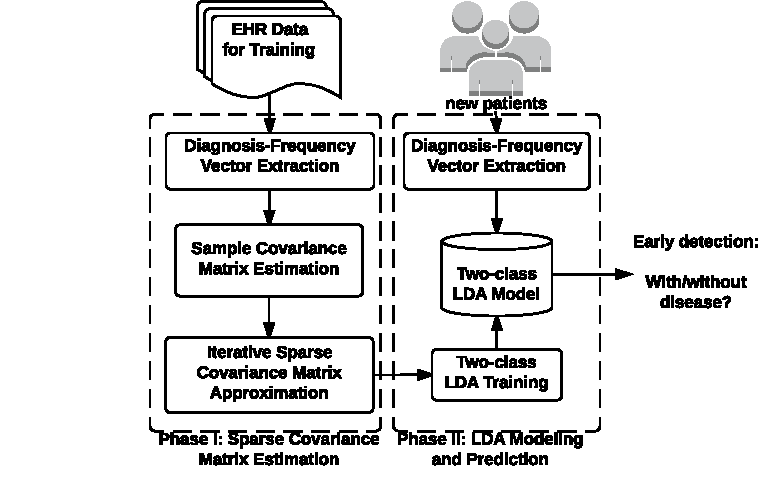
\includegraphics[width=0.48\textwidth]{./img/daehr.pdf}
\end{center}
\caption{\TheName\ Framework}
\end{figure}


\subsection{\TheName\ Framework}
In this section, we introduce the framework design of \DIFdelbegin \DIFdel{\TheName. 
The framework of \TheName}%DIFDELCMD < \ %%%
\DIFdelend \DIFaddbegin \DIFadd{\TheName{}. 
\TheName{} }\DIFaddend consists of two phases\DIFdelbegin \DIFdel{, which first uses }\DIFdelend \DIFaddbegin \DIFadd{.  
First, we use }\DIFaddend the EHR data for training to estimate the covariance matrices used in LDA \DIFdelbegin \DIFdel{w.r.t }\DIFdelend \DIFaddbegin \DIFadd{with respect to }\DIFaddend our problem formulation\DIFdelbegin \DIFdel{, then adopts LDA with newly-estimated }\DIFdelend \DIFaddbegin \DIFadd{. 
Next, we adopt LDA with newly estimated }\DIFaddend parameters to predict \DIFdelbegin \DIFdel{if }\DIFdelend \DIFaddbegin \DIFadd{whether }\DIFaddend the new patient will develop the targeted disease.

\emph{Phase I: Sparse Covariance Matrix Estimation --- } Given the patients' EHR data as \DIFaddbegin \DIFadd{a }\DIFaddend training set, this phase estimates the sparse covariance matrices for two classes of patients with following two steps:
\begin{enumerate}
    \item \textbf{Diagnosis-frequency Vector Extraction and Sample Covariance Matrix Estimation --- } \DIFdelbegin \DIFdel{\TheName}%DIFDELCMD < \ %%%
\DIFdel{first convert }\DIFdelend \DIFaddbegin \DIFadd{\TheName{} first converts }\DIFaddend each patient's EHR data to a diagnosis-frequency vector and \DIFdelbegin \DIFdel{combine }\DIFdelend \DIFaddbegin \DIFadd{combines }\DIFaddend it with his/her label (indicating \DIFdelbegin \DIFdel{if }\DIFdelend \DIFaddbegin \DIFadd{whether }\DIFaddend the patient has been diagnosed with \DIFdelbegin \DIFdel{/without }\DIFdelend the targeted disease)\DIFdelbegin \DIFdel{i.e. ,  }\DIFdelend \DIFaddbegin \DIFadd{. Specifically, we acquire }\DIFaddend $(X_0,l_0)\dots (X_{m-1},l_{m-1})$\DIFaddbegin \DIFadd{, }\DIFaddend where $l_i\in\{-1,+1\}$ \DIFdelbegin \DIFdel{as }\DIFdelend \DIFaddbegin \DIFadd{is }\DIFaddend the label of the $i^{th}$ patient. With the vectors \DIFdelbegin \DIFdel{of }\DIFdelend \DIFaddbegin \DIFadd{corresponding to each of the }\DIFaddend two classes, \DIFdelbegin \DIFdel{\TheName}%DIFDELCMD < \ %%%
\DIFdelend \DIFaddbegin \DIFadd{\TheName{} }\DIFaddend then estimates the sample covariance matrices for the two classes $\Sigma_+$ and $\Sigma_-$ using \DIFdelbegin \DIFdel{Eq.}\DIFdelend \DIFaddbegin \DIFadd{Equation}\DIFaddend ~\ref{eq:sample-cov}.

    \item \textbf{Iterative Sparse Covariance Matrix Approximation --- } Given sample covariance matrices $\Sigma_+$ and $\Sigma_-$, \DIFdelbegin \DIFdel{\TheName}%DIFDELCMD < \ %%%
\DIFdelend \DIFaddbegin \DIFadd{\TheName{} }\DIFaddend estimates the positive-definite $\ell^1$-penalized estimation of both $\Sigma_+$ and $\Sigma_-$ using a unified iterative approximation process, where \DIFdelbegin \DIFdel{\TheName}%DIFDELCMD < \ %%%
\DIFdelend \DIFaddbegin \DIFadd{\TheName{} }\DIFaddend treats $\Sigma_+$ and $\Sigma_-$ equally. 
    As shown in \DIFdelbegin \DIFdel{Alg.}\DIFdelend \DIFaddbegin \DIFadd{Algorithm}\DIFaddend ~\ref{alg:iap}, given an input sample covariance matrix $\Sigma_0=\Sigma_+$ or $\Sigma_-$, the process iteratively approximates to the positive definite $\ell^1$-penalized estimation of $\Sigma_0$ \DIFdelbegin \DIFdel{, through alternating two algorithms --- }\DIFdelend \DIFaddbegin \DIFadd{through alternating between two algorithms---}\DIFaddend \emph{$\ell^1$-penalized Sparse Matrix Estimation} and \emph{Nearest Positive \DIFdelbegin \DIFdel{Semi-Definite }\DIFdelend \DIFaddbegin \DIFadd{Semidefinite }\DIFaddend Matrix Approximation} in each iteration. In \DIFdelbegin \DIFdel{Alg}\DIFdelend \DIFaddbegin \DIFadd{Algorithm}\DIFaddend ~\ref{alg:iap}, $\Delta'=\frac{||\Sigma_{t+1}-\Sigma_{t}||_\infty}{||\Sigma_{t}||_\infty}$ and $tol$ is a threshold characterizing the tolerance of convergence. 
    Specifically, in each (\DIFdelbegin \DIFdel{e.g}\DIFdelend \DIFaddbegin \DIFadd{i.e}\DIFaddend ., the $t^{th}$, $t\geq 0$) iteration\DIFdelbegin \DIFdel{iteration}\DIFdelend , the process obtains an improved result $\Sigma_{t+1}$ using the previous result $\Sigma_{t}$. 
    With the result improved \DIFdelbegin \DIFdel{iteration by }\DIFdelend \DIFaddbegin \DIFadd{each }\DIFaddend iteration, the algorithm stops only when the predefined convergence \DIFdelbegin \DIFdel{achieved }\DIFdelend \DIFaddbegin \DIFadd{is achieved (}\DIFaddend $\Delta''< tol$\DIFdelbegin \DIFdel{or maximal iterations reached }\DIFdelend \DIFaddbegin \DIFadd{) or after iterating $maxit'$ times (i.e., }\DIFaddend $t>maxit'$\DIFaddbegin \DIFadd{)}\DIFaddend .


\end{enumerate}
\DIFdelbegin \DIFdel{Please note }\DIFdelend \DIFaddbegin \DIFadd{Note }\DIFaddend that the covariance matrices for the two classes of patients are estimated in this phase through \DIFdelbegin \DIFdel{an unified process, we }\DIFdelend \DIFaddbegin \DIFadd{a unified process.
We }\DIFaddend denote the new covariance matrices as $\Sigma_+^*$ and $\Sigma_-^*$ for the positive and negative classes\DIFaddbegin \DIFadd{, }\DIFaddend respectively.

\begin{algorithm}
\caption{Iterative Approximation Process for Sparse Covariance Matrix Estimation}
\label{alg:iap}
\DIFdelbegin %DIFDELCMD < \KwData{$\Sigma_{0}$ -- the sample covariance matrix i.e., $\Sigma_+$ or $\Sigma_-$}
%DIFDELCMD < \KwResult{${\Sigma_{t+1}}$ -- the positive definite $\ell^1$-penalized estimation of $\Sigma_0$}
%DIFDELCMD < \Begin{
%DIFDELCMD < \While{ $\Delta' \geq tol, \text{ or }0\leq t \leq maxit'$  }{
%DIFDELCMD < 	$\Sigma_{t+\frac{1}{2}}\gets \ell^1$-penalized sparse estimation of $\Sigma_t$
%DIFDELCMD <     $\Sigma_{t+1}\gets $ the nearest positive semi-definite approximation to  $\Sigma_{t+\frac{1}{2}}$
%DIFDELCMD < }
%DIFDELCMD < \Return{$\Sigma_{t+1}$}
%DIFDELCMD < }
%DIFDELCMD < %%%
\DIFdelend \DIFaddbegin \KwData{$\Sigma_{0}$ --- the sample covariance matrix i.e., $\Sigma_+$ or $\Sigma_-$}
\KwResult{${\Sigma_{t+1}}$ --- the positive definite $\ell^1$-penalized estimation of $\Sigma_0$}
\Begin{
\While{ $\Delta' \geq tol, \text{ or }0\leq t \leq maxit'$  }{
	$\Sigma_{t+\frac{1}{2}}\gets \ell^1$-penalized sparse estimation of $\Sigma_t$
    $\Sigma_{t+1}\gets $ the nearest positive semidefinite approximation to  $\Sigma_{t+\frac{1}{2}}$
}
\Return{$\Sigma_{t+1}$}
}
\DIFaddend \end{algorithm}


\emph{Phase II: LDA Modelling and Prediction --- } Given the two estimated matrices $\Sigma_+$ and $\Sigma_-$ as well as the training samples, this phase first trains the optimal model for LDA prediction\DIFdelbegin \DIFdel{and then }\DIFdelend \DIFaddbegin \DIFadd{. 
Then, it }\DIFaddend uses the LDA model for new \DIFdelbegin \DIFdel{patients }\DIFdelend \DIFaddbegin \DIFadd{patient }\DIFaddend prediction. 
This phase consists of following two steps:
\begin{enumerate}
    \item \textbf{LDA Model Training --- } Given the two estimated covariance matrices $\Sigma_+^*$ and $\Sigma_-^*$ as well as training samples $(X_0,l_0)\dots (X_{m-1},l_{m-1})$, \DIFdelbegin \DIFdel{\TheName}%DIFDELCMD < \ %%%
\DIFdel{searches }\DIFdelend \DIFaddbegin \DIFadd{\TheName{} searches for }\DIFaddend the optimal threshold $T^*$ that can maximally classify the two classes of samples \DIFdelbegin \DIFdel{with Eq.}\DIFdelend \DIFaddbegin \DIFadd{using Equation}\DIFaddend ~\ref{eq:glda}. 
        In this case, \DIFdelbegin \DIFdel{\TheName}%DIFDELCMD < \ %%%
\DIFdel{models }\DIFdelend \DIFaddbegin \DIFadd{\TheName{} uses }\DIFaddend a LDA model as $(\Sigma_+^*,\mu_+,\Sigma_-^*,\mu_-,T^*)$.
    \item \textbf{LDA-based new Patient Prediction --- } Given a new patient's EHR data, \DIFdelbegin \DIFdel{\TheName}%DIFDELCMD < \ %%%
\DIFdel{first convert }\DIFdelend \DIFaddbegin \DIFadd{\TheName{} first converts }\DIFaddend her data to \DIFaddbegin \DIFadd{a }\DIFaddend diagnosis-frequency vector \DIFaddbegin \DIFadd{(}\DIFaddend e.g., $X'$\DIFdelbegin \DIFdel{. 
Then together }\DIFdelend \DIFaddbegin \DIFadd{). 
        Combined }\DIFaddend with the LDA model described as $(\Sigma_+^*,\mu_+,\Sigma_-^*,\mu_-,T^*)$, \DIFdelbegin \DIFdel{\TheName}%DIFDELCMD < \ %%%
\DIFdel{predict if }\DIFdelend \DIFaddbegin \DIFadd{\TheName{} predicts whether }\DIFaddend the patient will develop the targeted disease using the criterion in \DIFdelbegin \DIFdel{Eq.}\DIFdelend \DIFaddbegin \DIFadd{Equation}\DIFaddend ~\ref{eq:glda}.
\end{enumerate}
%

After \DIFaddbegin \DIFadd{the }\DIFaddend above two phases terminate, \DIFdelbegin \DIFdel{\TheName}%DIFDELCMD < \ %%%
\DIFdel{has }\DIFdelend \DIFaddbegin \DIFadd{\TheName{} will have (1) }\DIFaddend learned a LDA model with advanced covariance \DIFdelbegin \DIFdel{matrices estimation, then }\DIFdelend \DIFaddbegin \DIFadd{matrix estimation, and (2)  }\DIFaddend adopted the LDA model to enable the early detection of targeted disease. 
Though the \DIFdelbegin \DIFdel{whole framework has beens sketched}\DIFdelend \DIFaddbegin \DIFadd{architecture of the framework is discussed here}\DIFaddend , the design of \DIFdelbegin \DIFdel{some algorithms have not yet been introduced.
The design of }\DIFdelend \DIFaddbegin \DIFadd{the }\DIFaddend aforementioned \emph{$\ell^1$-penalized Sparse Matrix Estimation} and \emph{Nearest Positive Semi-Definite Matrix Approximation} algorithms are discussed in following sections.


\section{\TheName\ Core Algorithms}~\label{sec:4}
In this section, we first introduce the two core algorithm used in \TheName, then analyzes the performance of the proposed algorithms.

\subsection{$\ell^1$-penalized Sparse Matrix Estimation}
Given the covariance matrix estimated in the previous iteration $\Sigma_{t}$, this algorithm estimates $\Sigma_{t+\frac{1}{2}}$ -- the $\ell^1$-penalized sparse estimation of $\Sigma_{t}$, using the Proximal Gradient Descent algorithm~\cite{nesterov2004introductory} with following objective function:   
\begin{equation}
\emph{min. }\frac{1}{2}||\Sigma_{t+\frac{1}{2}}-\Sigma_t||_F^2+\tau |\Sigma_{t+\frac{1}{2}}|_1,
\label{eq:sparse-imp}
\end{equation}
where $\tau$ is a Lagrange multiplier~\cite{wu2009karush}. When $\tau\geq 0$, the Eq.~\ref{eq:sparse-imp} is a \emph{convex function with sparse input} which can be optimally converged using proximal gradient descent~\cite{nesterov2004introductory}. Please note that $\Sigma_{t+\frac{1}{2}}$ is neither symmetric nor positive semi-definite.



\subsection{Nearest Positive Semi-Definite Matrix Approximation}
Given the sparse matrix $\Sigma_{t+\frac{1}{2}}$, we intend to approximate its nearest positive-definite matrix $\Sigma_{t}$ (the output of the $t^{th}$ iteration) as Equation~\ref{eq:nearest-pd}. 
%
\begin{equation}
\emph{min. } ||\Sigma_{t+1}-\Sigma_{t+\frac{1}{2}}||_F^2 \emph{ s.t. }\Sigma_{t+1}\in  {\bf }I^+
\label{eq:nearest-pd}
\end{equation}
%
In order to achieve the goal, we use the Alternating Projection Algorithm~\cite{higham2002computing} shown in Alg~\ref{alg:apm}. Specifically, the projection $P_S(A)=\frac{1}{2}(V\lambda_+V^T+(V\lambda_+V^T)^T)$ and  $\lambda_+=\langle min\{\lambda_0,0\},min\{\lambda_1,0\}\dots  \rangle$, where $V,\lambda_i$ is the eigenvalue decomposition of $A$; the projection $P_U(A)=A'$, where $A'_{i,j}=1$ when $i=j,$ and $A'_{i,j}=A_{i,j}$ when $i\neq j$; the stopping criterion $\Delta''=max\{\frac{||H_{k+1}-H_k||_\infty}{||H_k||_\infty}, \frac{||H_{k+1}^*-H_k^*||_\infty}{||H_k^*||_\infty}, \frac{||H_{k+1}^*-H_k^*||_\infty}{||H_k||_\infty}\}$.


The algorithm stops when the predefined convergence achieved $\Delta'' < tol$, or maximal iterations reached $k= maxit''$. Please note that when the algorithm stops at any $k> 0$, the output $\Sigma_{t+1}$ must be a positive semi-definite matrix; while when $k\to+\infty$, the output $\Sigma_{t+1}$ could converge to the optimal solution~\cite{dykstra1983algorithm} of the optimization problem addressed in Eq.~\ref{eq:nearest-pd}.

\begin{algorithm}
\caption{Alternating Projection Algorithm for Nearest Positive Definite Matrix Approximation}
\label{alg:apm}
\KwData{$\Sigma_{t+\frac{1}{2}}$ -- the $\ell^1$-penalized sparse estimation of $\Sigma_{t}$, $tol$ -- the tolerance of convergence}
\KwResult{$\Sigma_{t+1}$ -- the nearest positive definite approximation to $\Sigma_{t+\frac{1}{2}}$}
\Begin{
 {\bf initialization:}\\
  $H_0$ = $\frac{1}{2}(\Sigma_{t+\frac{1}{2}}+\Sigma_{t+\frac{1}{2}}^T)$, $k = 1$, $I_{mod_0} = 0$, $\Delta = 1$;\\
\While{ $\Delta'' \geq tol, \text{ or } 0\leq k \leq maxit''$  }{
 $R_{k+1} = H_{k} - I_{mod_{k}}$, \\%\% $I_{mod_{k-1}}$ is Dykstra's correction;\\
 $H_{k+1}^{*} = P_S(R_{k+1})$;\\
 $I_{mod_{k+1}} = H_{k+1}^{*} - R_{k+1}$;\\
 $H_{k+1} = P_U(H_{k+1}^{*})$;
}
$\Sigma_{t+1}=H_{k+1}$\\
\Return{$\Sigma_{t+1}$}
}
\end{algorithm}


\subsection{Algorithm Analysis}
\DIFdelbegin %DIFDELCMD < 

%DIFDELCMD < %%%
\DIFdelend \section{Evaluation}\label{sec:5}
% why study mental health disorders?
In this section, we \DIFdelbegin \DIFdel{first introduce the experiment }\DIFdelend \DIFaddbegin \DIFadd{introduce the experimental }\DIFaddend design of our evaluation\DIFdelbegin \DIFdel{, then we introduce the experiment }\DIFdelend \DIFaddbegin \DIFadd{.
Then, we present the experimental }\DIFaddend results, including the performance comparison between \DIFdelbegin \DIFdel{\TheName}%DIFDELCMD < \ %%%
\DIFdelend \DIFaddbegin \DIFadd{the \TheName{} framework }\DIFaddend and original LDA baselines\DIFdelbegin \DIFdel{, as well as the performance comparison between \TheName}%DIFDELCMD < \ %%%
\DIFdelend \DIFaddbegin \DIFadd{.
Additionally, we present performance comparisons between \TheName{} }\DIFaddend and other predictive models. 
Finally, we compare the time \DIFdelbegin \DIFdel{consumption of \TheName}%DIFDELCMD < \ %%%
\DIFdel{to }\DIFdelend \DIFaddbegin \DIFadd{consumed by \TheName{} with }\DIFaddend other models.

\subsection{\DIFdelbegin \DIFdel{Experiment }\DIFdelend \DIFaddbegin \DIFadd{Experimental }\DIFaddend Design}
We first present the datasets used for \DIFdelbegin \DIFdel{\TheName}%DIFDELCMD < \ %%%
\DIFdelend \DIFaddbegin \DIFadd{our }\DIFaddend evaluation, then introduce the targeted diseases for the early detection\DIFdelbegin \DIFdel{, further we }\DIFdelend \DIFaddbegin \DIFadd{.  We also }\DIFaddend specify the settings of early detection.

\textbf{Dataset for Evaluation \DIFdelbegin \DIFdel{- }\DIFdelend \DIFaddbegin \DIFadd{--- }\DIFaddend } In this study, to evaluate \DIFdelbegin \DIFdel{\TheName}\DIFdelend \DIFaddbegin \DIFadd{\TheName{}}\DIFaddend , we plan use the de-identified EHR data from the College Health Surveillance Network (CHSN)\DIFaddbegin \DIFadd{, }\DIFaddend which contains over 1 million patients and 6 million visits from 31 student health centers across the \DIFdelbegin \DIFdel{US}\DIFdelend \DIFaddbegin \DIFadd{United States}\DIFaddend ~\cite{turner_college_2015}. 
In the experiments, we use the EHR data from 10 participating schools. 
The available information includes ICD-9 diagnostic codes, CPT procedural codes\DIFaddbegin \DIFadd{, }\DIFaddend and limited demographic information. There are over 200,000 enrolled students in those 10 schools representing all geographic regions of the US. The demography of enrolled students (sex, race/ethnicity, age, undergraduate/graduate status) closely matched the demography for the population of US universities.

%DIF >  KJL I can see a reviewer being upset with the criteria for "other related disorders".
\textbf{Targeted Disease for Early Detection \DIFdelbegin \DIFdel{- }\DIFdelend \DIFaddbegin \DIFadd{--- }\DIFaddend } Among all diseases recorded in CHSN, we choose mental health disorders, including \emph{anxiety disorders, mood disorders, depression disorders\DIFaddbegin \DIFadd{, }\DIFaddend and other related disorders}, as the targeted disease for early detection. Specifically, we plan to evaluate \DIFdelbegin \DIFdel{\TheName}%DIFDELCMD < \ %%%
\DIFdelend \DIFaddbegin \DIFadd{\TheName{} }\DIFaddend using the early detection of mental health disorders in \emph{college students}, considering following issues:
\begin{enumerate}
\item  \emph{\DIFdelbegin \DIFdel{Emergency }\DIFdelend \DIFaddbegin \DIFadd{Emergence }\DIFaddend of early detection of mental health disorders \DIFdelbegin \DIFdel{- }\DIFdelend \DIFaddbegin \DIFadd{--- }\DIFaddend } Mental health disorders have become a severe problem in the United States and many other countries that 18.6\% adults \DIFdelbegin \DIFdel{are with }\DIFdelend \DIFaddbegin \DIFadd{have }\DIFaddend at least one mental \DIFdelbegin \DIFdel{disorders}\DIFdelend \DIFaddbegin \DIFadd{disorder}\DIFaddend . 
According to the Spring 2014 American College Health Association's National College Health Assessment report, approximately half of the college students have had the feeling of hopeless and overwhelming anxiety~\cite{ACHA2014}. 

\item  \emph{Difficulty \DIFdelbegin \DIFdel{to recognize }\DIFdelend \DIFaddbegin \DIFadd{recognizing }\DIFaddend mental health disorders in early \DIFdelbegin \DIFdel{stage - }\DIFdelend \DIFaddbegin \DIFadd{stages --- }\DIFaddend } Mental health disorders are \DIFdelbegin \DIFdel{unrecognized frequently }\DIFdelend \DIFaddbegin \DIFadd{frequently unrecognized  }\DIFaddend in primary care\DIFdelbegin \DIFdel{that untimely }\DIFdelend \DIFaddbegin \DIFadd{. 
Untimely }\DIFaddend treatment results in emotional, physical, economic, and social burdens to patients and others. 

\item \emph{\DIFdelbegin \DIFdel{Limitation }\DIFdelend \DIFaddbegin \DIFadd{Limitations }\DIFaddend of common approaches \DIFdelbegin \DIFdel{to }\DIFdelend \DIFaddbegin \DIFadd{for }\DIFaddend early detection of mental health disorders \DIFdelbegin \DIFdel{- }\DIFdelend \DIFaddbegin \DIFadd{--- }\DIFaddend } Questionnaires are commonly used to detect mental health disorders. 
    Usually, specific questionnaires, interviews, or standard \DIFdelbegin \DIFdel{measurement }\DIFdelend \DIFaddbegin \DIFadd{measurements }\DIFaddend are designed by researchers to collect patients' behavioral information targeting \DIFdelbegin \DIFdel{on }\DIFdelend a particular psychiatric disorder. 
    In particular, psychological screening, PHQ-9, is used to evaluate a patient's risk of mental health disorders~\cite{kroenke2002phq}. However, these approaches are not generally applicable in primary care thus cannot detect mental disorders at an early stage. 

\end{enumerate}
%
\DIFdelbegin \DIFdel{With all above in mind, we }\DIFdelend \DIFaddbegin \DIFadd{We }\DIFaddend are motivated to use EHR data for the early detection of mental health disorders, considering the accessibility and information contained in EHR \DIFaddbegin \DIFadd{data}\DIFaddend . 

\textbf{Early Detection Settings \DIFdelbegin \DIFdel{- }\DIFdelend \DIFaddbegin \DIFadd{--- }\DIFaddend } From the CHSN datasets, we select 21,097 patients with anxiety/depression in the target group and 327,198 patients without any mental health disorder in the control group. 
We represent each patient using his/her diagnosis-frequency vector based on the clustered codeset, where four clustered codes (i.e., xxx, xxx, xxx, xxx) are considered to represent the diagnoses of mental health disorders. 
Specifically, if a patient has any of these four codes in his/her EHR, we \DIFdelbegin \DIFdel{consider }\DIFdelend \DIFaddbegin \DIFadd{say that }\DIFaddend he/she has been diagnosed with mental health disorders as ground truth.
\DIFdelbegin \DIFdel{Please note }\DIFdelend \DIFaddbegin \DIFadd{Note }\DIFaddend that in our research, we \DIFdelbegin \DIFdel{don't }\DIFdelend \DIFaddbegin \DIFadd{do not }\DIFaddend intend to predict these four types of mental disorders separately, as these four disorders are usually correlated and heavily overlapped in clinical practices.
%DIF >  KJL might want a citation for that last sentence

\begin{table*}
{
\begin{center}
\caption{Performance Comparison between \TheName\ and LDA Baselines (Testing Sample Size =$200\times 2$)}
		\label{tab:table11}
\begin{tabular}{*{10}{c}}
\toprule
    & & \multicolumn{8}{c}{Training Set $\times 2$}\\
    \cmidrule(lr){3-10}
    & & 
    \multicolumn{2}{c}{50} &
  %  \multicolumn{3}{c}{100} &
    \multicolumn{2}{c}{150} &
  % \multicolumn{3}{c}{200} &
    \multicolumn{2}{c}{250} &
  % \multicolumn{3}{c}{300} &
    \multicolumn{2}{c}{350} \\
\cmidrule(lr){3-4}
\cmidrule(lr){5-6}
\cmidrule(lr){7-8}
\cmidrule(lr){9-10}
Algorithm & Parameters & \texttt{Accuracy} & \texttt{F1-Score} & 
									   	 \texttt{Accuracy} & \texttt{F1-Score} & 
                          			 \texttt{Accuracy} & \texttt{F1-Score} & 
                           			 \texttt{Accuracy} & \texttt{F1-Score} \\
 \cmidrule(lr){1-2}                        
\cmidrule(lr){3-4}
\cmidrule(lr){5-6}
\cmidrule(lr){7-8}
\cmidrule(lr){9-10}
    LDA & N/A &   0.547 & 0.539   &     0.617 & 0.612       & 0.639 & 0.644      & 0.661 & 0.670 \\

\cmidrule(lr){1-2}                        
\cmidrule(lr){3-4}
\cmidrule(lr){5-6}
\cmidrule(lr){7-8}
\cmidrule(lr){9-10}
    DIAG & N/A &   0.592 & 0.591 &      0.635 & 0.635 &      0.639 & 0.639&   0.653 & 0.660    \\
   % \midrule
    \cmidrule(lr){1-2}                        
\cmidrule(lr){3-4}
\cmidrule(lr){5-6}
\cmidrule(lr){7-8}
\cmidrule(lr){9-10}

    \multirow{3}{*}{Shrinkage($\beta$)} 
& 0.25 &   0.593& 0.592 &      0.636 & 0.638      & 0.640 & 0.643      & 0.656 & 0.665      \\
& 0.50 &   0.594 & 0.592 &      0.630 & 0.630    & 0.641 & 0.645     & 0.660 & 0.669     \\
& 0.75 &   0.592 & 0.590 &      0.626 & 0.624    & 0.639 & 0.643      & 0.662 & 0.672   \\
    % \midrule
\cmidrule(lr){1-2}                        
\cmidrule(lr){3-4}
\cmidrule(lr){5-6}
\cmidrule(lr){7-8}
\cmidrule(lr){9-10}
     \multirow{5}{*}{\TheName($\tau$)} 
     & $0.005*0.5^{0}$ &   0.644 & 0.692 &     \textbf{0.667} & 0.714      & \textbf{0.662} & \textbf{0.716}     & \textbf{0.670} & \textbf{0.722}    \\
     & $0.005*0.5^{1}$ &   0.645 & 0.694 &     0.666 & 0.713      & \textbf{0.662} & \textbf{0.716}    & \textbf{0.670} & \textbf{0.722}    \\     
     & $0.005*0.5^{2}$ &   \textbf{0.646} & \textbf{0.697} &  0.663 & 0.714      & \textbf{0.662} & \textbf{0.716}     & \textbf{0.670} & \textbf{0.722}  \\
     & $0.005*0.5^{3}$ &   \textbf{0.646} & 0.694 &     0.661 & 0.712     & \textbf{0.662} & \textbf{0.716}     & \textbf{0.670} & \textbf{0.722}   \\
     & $0.005*0.5^{4}$ &   \textbf{0.646} & 0.696 &     0.662 & \textbf{0.715}     & \textbf{0.662} & \textbf{0.716}     & \textbf{0.670} & \textbf{0.722}  \\

     \bottomrule

\end{tabular}

\end{center}
}
\end{table*}


\begin{table*}
{
\begin{center}
\caption{Performance Comparison between \TheName\ and LDA Baselines  (Testing Sample Size =$1000\times 2$)}
		\label{tab:table12}
\begin{tabular}{*{10}{c}}
\toprule
    & & \multicolumn{8}{c}{Training Set $\times 2$}\\
    \cmidrule(lr){3-10}
    & & 
    \multicolumn{2}{c}{50} &
  %  \multicolumn{3}{c}{100} &
    \multicolumn{2}{c}{150} &
  % \multicolumn{3}{c}{200} &
    \multicolumn{2}{c}{250} &
  % \multicolumn{3}{c}{300} &
    \multicolumn{2}{c}{350} \\
\cmidrule(lr){3-4}
\cmidrule(lr){5-6}
\cmidrule(lr){7-8}
\cmidrule(lr){9-10}
Algorithm & Parameters & \texttt{Accuracy} & \texttt{F1-Score} &
						\texttt{Accuracy} & \texttt{F1-Score} &
                           \texttt{Accuracy} & \texttt{F1-Score}  &
                           \texttt{Accuracy} & \texttt{F1-Score}  \\
 \cmidrule(lr){1-2}                        
\cmidrule(lr){3-4}
\cmidrule(lr){5-6}
\cmidrule(lr){7-8}
\cmidrule(lr){9-10}
    LDA & N/A &   0.552 & 0.545  &     0.619 & 0.620      & 0.644 & 0.648      & 0.656 & 0.663  \\

     \cmidrule(lr){1-2}                        
\cmidrule(lr){3-4}
\cmidrule(lr){5-6}
\cmidrule(lr){7-8}
\cmidrule(lr){9-10}
    DIAG & N/A &   0.595 & 0.588  &     0.624 & 0.625      & 0.641 & 0.642     & 0.653 & 0.662  \\
   % \midrule
    \cmidrule(lr){1-2}                        
\cmidrule(lr){3-4}
\cmidrule(lr){5-6}
\cmidrule(lr){7-8}
\cmidrule(lr){9-10}

    \multirow{3}{*}{Shrinkage($\beta$)} 

& 0.25 &   0.596 & 0.592  &     0.629 & 0.631     & 0.644 & 0.648      & 0.657 & 0.667     \\   			& 0.50 &   0.594 & 0.589 &     0.630 & 0.633      & 0.646 & 0.649     & 0.660 & 0.670     \\
& 0.75 &   0.590 & 0.584  &     0.629 & 0.632     & 0.647 & 0.650     & 0.660 & 0.668     \\
    % \midrule
     \cmidrule(lr){1-2}                        
\cmidrule(lr){3-4}
\cmidrule(lr){5-6}
\cmidrule(lr){7-8}
\cmidrule(lr){9-10}
     \multirow{5}{*}{\TheName($\tau$)} 
     & $0.005*0.5^{0}$ &   0.653 & 0.711 &     \textbf{0.655} & \textbf{0.716}      & 0.666 & 0.718     & \textbf{0.667} & \textbf{0.720}    \\
     & $0.005*0.5^{1}$ &   0.653 & 0.711  &     \textbf{0.655} & \textbf{0.716}      & 0.666 & 0.718      & \textbf{0.667} & \textbf{0.720}   \\     
     & $0.005*0.5^{2}$ &   \textbf{0.653} & \textbf{0.712} &     \textbf{0.655} & \textbf{0.716}      & 0.666 & \textbf{0.720}     & \textbf{0.667} & \textbf{0.720}  \\
     & $0.005*0.5^{3}$ &   0.652 & 0.710  &     \textbf{0.655} & \textbf{0.716}      & 0.666 & 0.719     &\textbf{0.667} & \textbf{0.720}    \\
     & $0.005*0.5^{4}$ &   0.652 & 0.710  &     \textbf{0.655} & \textbf{0.716}       & \textbf{0.667} & \textbf{0.720}     & \textbf{0.667} & \textbf{0.720}    \\     
     \bottomrule

\end{tabular}
\end{center}}
\end{table*}


\subsection{Comparison to LDA Baselines}\label{sec:baselines}
In order to understand the performance improvement of \DIFdelbegin \DIFdel{\TheName}%DIFDELCMD < \ %%%
\DIFdelend \DIFaddbegin \DIFadd{\TheName{} }\DIFaddend beyond classic LDA, we first propose three LDA baseline approaches that we compare \DIFdelbegin \DIFdel{to \TheName}\DIFdelend \DIFaddbegin \DIFadd{against \TheName{}}\DIFaddend :
\begin{itemize}
\item \textbf{LDA} \DIFdelbegin \DIFdel{- }\DIFdelend \DIFaddbegin \DIFadd{--- }\DIFaddend This algorithm is based on the common implementation of generalized linear discriminant analysis using sample covariance matrix estimation and \DIFdelbegin \DIFdel{Eq.}\DIFdelend \DIFaddbegin \DIFadd{Equation}\DIFaddend ~\ref{eq:glda}. \DIFdelbegin \DIFdel{To handle the singular covariance matrices, this algorithm uses }\DIFdelend \DIFaddbegin \DIFadd{This algorithm uses the }\DIFaddend pseudo-inverse~\cite{ye2004optimization} to replace \DIFaddbegin \DIFadd{the }\DIFaddend matrix inverse in \DIFdelbegin \DIFdel{Eq.~\ref{eq:glda} , }\DIFdelend \DIFaddbegin \DIFadd{Equation~\ref{eq:glda} }\DIFaddend when the sample covariance matrix is singular.

\item \textbf{Shrinkage \DIFdelbegin \DIFdel{- }\DIFdelend \DIFaddbegin \DIFadd{--- }\DIFaddend } This algorithm is based on the aforementioned \textbf{LDA} implementation (using pseudo-inverse). However, rather than using the sample covariance matrix, this algorithm adopts the sparse estimation of the covariance matrix $\Sigma^*=\beta*\Sigma+(1-\beta) * diag(\Sigma)$, where $\Sigma$ refers to the given sample covariance matrix, $diag(\Sigma)$ refers to a $p\times p$ matrix preserving the diagonal elements of $\Sigma$ only, and $\beta\geq 0$ is a tuning parameter. 
    \DIFdelbegin \textbf{\DIFdel{Shrinkage}} %DIFAUXCMD
\DIFdelend \DIFaddbegin \DIFadd{The Shrinkage }\DIFaddend algorithm can be considered as a heuristic approach to the optimization problem addressed in \DIFdelbegin \DIFdel{Eq.}\DIFdelend \DIFaddbegin \DIFadd{Equation}\DIFaddend ~\ref{eq:problem}.

\item \textbf{DIAG \DIFdelbegin \DIFdel{- }\DIFdelend \DIFaddbegin \DIFadd{--- }\DIFaddend } This algorithm is based on the \DIFdelbegin \textbf{\DIFdel{Shrinkage}} %DIFAUXCMD
\DIFdelend \DIFaddbegin \DIFadd{Shrinkage approach }\DIFaddend with $\beta=0.0$, which means the sparse estimation of the covariance matrix $\Sigma^*=diag(\Sigma)$ used in LDA only includes the diagonal information of the sample covariance matrix.

\end{itemize}
\DIFdelbegin \DIFdel{Please note }\DIFdelend \DIFaddbegin \DIFadd{Note }\DIFaddend that the implementation of \DIFdelbegin \DIFdel{\TheName}%DIFDELCMD < \ %%%
\DIFdelend \DIFaddbegin \DIFadd{\TheName{} }\DIFaddend as well as above baselines are derived from the Java implementation of LDA released by Psychometrica\footnote{Java-Implementation of the Linear Discriminant Analysis, Institute for Psychological Diagnosis, http://www.psychometrica.de/lda.html}.

With the four algorithms, we perform experiments with following settings:
\begin{itemize}
\item \textbf{Training Samples \DIFdelbegin \DIFdel{- }\DIFdelend \DIFaddbegin \DIFadd{--- }\DIFaddend } we randomly select 50, 100, 150, 200, 250, 300, 350, and 400 patients from the target group as the positive training samples, then randomly select the same number of patients from \DIFaddbegin \DIFadd{the }\DIFaddend control group as negative training samples; here, the training set of the two classes of patients is balanced\DIFdelbegin \DIFdel{;
}\DIFdelend \DIFaddbegin \DIFadd{.
}\DIFaddend \item \textbf{Testing Samples \DIFdelbegin \DIFdel{- }\DIFdelend \DIFaddbegin \DIFadd{--- }\DIFaddend } we randomly select 200 and 1000 unselected patients (not included in the training set) from the target group as well as the same number of unselected patients from \DIFaddbegin \DIFadd{the }\DIFaddend control group as \DIFaddbegin \DIFadd{the }\DIFaddend testing set; here, the testing set is also balanced.
\end{itemize}
%
For each setting, we \DIFdelbegin \DIFdel{evaluate }\DIFdelend \DIFaddbegin \DIFadd{execute }\DIFaddend the four algorithms and repeat 30 times. 
\DIFdelbegin \DIFdel{Particularly}\DIFdelend \DIFaddbegin \DIFadd{In particular}\DIFaddend , we are interested in measuring following metrics: 
\begin{equation}
\begin{aligned}
&Accuracy=\frac{TP+TN}{TP+TN+FP+FN},\\
&\text{F1-score}=\frac{2*TP}{2*TP+FP+FN}
\end{aligned}
\end{equation}
where $TP$, $TN$, $FP$, and $FN$ refer to the true-positive, true-negative, false-positive, and false-negative classification samples in early detection of mental health disorders respectively. 
Specifically, the \DIFdelbegin \DIFdel{metric Accuracy characterizes }\DIFdelend \DIFaddbegin \DIFadd{Accuracy metric characterizes the }\DIFaddend proportion of patients who are accurately classified in the early detection of mental disorders\DIFdelbegin \DIFdel{; while }\DIFdelend \DIFaddbegin \DIFadd{.  The }\DIFaddend F1-Score measures both correctness and completeness of the early detection. 

Table~\ref{tab:table11} and \DIFaddbegin \DIFadd{Table}\DIFaddend ~\ref{tab:table12} present \DIFdelbegin \DIFdel{a part of }\DIFdelend \DIFaddbegin \DIFadd{part of the }\DIFaddend comparison results. 
The results show that under all settings\DIFdelbegin \DIFdel{\TheName}%DIFDELCMD < \ %%%
\DIFdel{outperform }\DIFdelend \DIFaddbegin \DIFadd{, \TheName{} outperforms }\DIFaddend the three baseline algorithms in terms of overall accuracy and F1-score. 
%LDA:
% accuracy for testSample200: 18.1%, 8.1%, 3.6%, 1.4%, accuracy for testSample1000: 18.3%, 5.8%, 3.6%, 1.7%
% F1-score for testSample200:  29.3%, 16.8%, 11.2%, 7.6%, F1-score for testSample1000: 29.0%, 15.5%,  11.1%,  8.6%
Compared to LDA, \DIFdelbegin \DIFdel{\TheName}%DIFDELCMD < \ %%%
\DIFdelend \DIFaddbegin \DIFadd{\TheName{} }\DIFaddend achieves 1.4\%--18.3\% higher accuracy   and 7.6\%--29.3\% higher F1-score. 
Compared to Shrinkage and DIAG, \DIFdelbegin \DIFdel{\TheName}%DIFDELCMD < \ %%%
\DIFdelend \DIFaddbegin \DIFadd{\TheName{} }\DIFaddend achieves 
 % DIAG: 
 %accuracy for testSample200: 9.1%, 5.0%, 3.6%,2.6%, , accuracy for testSample1000: 9.7%, 5.0%, 4.1%, 2.1%
 % F1-score for testSample200: 17.9%,12.6%,   12.1%, 9.4% , F1-score for testSample1000: 21.1%, 14.6%,12.2%, 8.8%
 % Shrinkage:(这个太多了而且都差不多,我就算了0.25的..)
%accuracy for testSample200: 8.9%, 4.9%, 3.4%, 2.1%, accuracy for testSample1000:9.6%, 4.1%, 3.6%, 1.5%
 % F1-score for testSample200: 17.7%, 12.1%,   11.4%, 8.6% , F1-score for testSample1000: 20.3%, 13.5%, 11.1%, 7.9%
1.5\%--9.7\% higher accuracy and 7.9\%--21.1\% higher F1-score. 

Further, it is \DIFdelbegin \DIFdel{obvious }\DIFdelend \DIFaddbegin \DIFadd{clear }\DIFaddend that decreasing the \DIFdelbegin \DIFdel{training samples, larger the improvement of }\DIFdelend \DIFaddbegin \DIFadd{quantity of training samples results in a larger improvement in }\DIFaddend accuracy and F1-score\DIFdelbegin \DIFdel{obtained}\DIFdelend . 
In this case, we can conclude that \DIFdelbegin \DIFdel{\TheName}%DIFDELCMD < \ %%%
\DIFdelend \DIFaddbegin \DIFadd{\TheName{} }\DIFaddend significantly improves the accuracy and F1-score from the classic LDA\DIFaddbegin \DIFadd{, }\DIFaddend especially when the training sample size is small\DIFdelbegin \DIFdel{; while \TheName}%DIFDELCMD < \ %%%
\DIFdelend \DIFaddbegin \DIFadd{. 
\TheName{} }\DIFaddend outperforms all other baselines derived from LDA \DIFdelbegin \DIFdel{, }\DIFdelend in terms of accuracy and F1-score. 

\begin{table}
\footnotesize{
\begin{center}
\caption{Performance Comparison between \TheName\ and other Predictive Models}
		\label{tab:table13_compressed}
\begin{tabular}{*{5}{c}}
\toprule
    &  \multicolumn{4}{c}{Training Set $ \times 2$}\\
    \cmidrule(lr){2-5}
    &  
    \multicolumn{2}{c}{50} &
  %  \multicolumn{3}{c}{100} &
    %\multicolumn{3}{c}{150} &
  % \multicolumn{3}{c}{200} &
    \multicolumn{2}{c}{250} \\
  % \multicolumn{3}{c}{300} &
    %\multicolumn{3}{c}{350} \\
\cmidrule(lr){2-3}
\cmidrule(lr){4-5}
%\cmidrule(lr){9-11}
%\cmidrule(lr){12-14}
Algorithm & \texttt{Accuracy} & \texttt{F1-Score}&
						%\texttt{Accuracy} & \texttt{SEN0.} & \texttt{SPE0.} &
                          % \texttt{Accuracy} & \texttt{SEN0.} & \texttt{SPE0.} &
                           \texttt{Accuracy} & \texttt{F1-Score} \\
 \cmidrule(lr){1-1}                        
 \cmidrule(lr){2-3}
\cmidrule(lr){4-5}
%\cmidrule(lr){9-11}
%\cmidrule(lr){12-14}
    LDA &   0.551 & 0.549  &     0.639 & 0.641  \\

     \cmidrule(lr){1-1}                        
 \cmidrule(lr){2-3}
\cmidrule(lr){4-5}
%\cmidrule(lr){9-11}
%\cmidrule(lr){12-14}
    Logit. Reg. &   0.614 & 0.521  &     0.615 & 0.501 \\

    \cmidrule(lr){1-1}                        
 \cmidrule(lr){2-3}
\cmidrule(lr){4-5}
%\cmidrule(lr){9-11}
%\cmidrule(lr){12-14}
    SVM  &   0.614 & 0.608 &     0.660 & 0.669  \\
   % \midrule
    \cmidrule(lr){1-1}                        
 \cmidrule(lr){2-3}
\cmidrule(lr){4-5}
%\cmidrule(lr){9-11}
%\cmidrule(lr){12-14}

   AdaBoost-10 &   0.643 & 0.599 &     0.629 & 0.538   \\   
   \cmidrule(lr){1-1}                        
 \cmidrule(lr){2-3}
\cmidrule(lr){4-5}
%\cmidrule(lr){9-11}
%\cmidrule(lr){12-14}

    AdaBoost-50 &    0.633 & 0.568 &     0.633 & 0.550       \\

    % \midrule
     \cmidrule(lr){1-1}                        
 \cmidrule(lr){2-3}
\cmidrule(lr){4-5}
%\cmidrule(lr){9-11}
%\cmidrule(lr){12-14}
    % \multirow{5}{*}{DAEHR($\lambda$)} 
     \TheName\ &  \textbf{0.658} & 0.695  &     \textbf{0.684} & 0.719      \\

     \bottomrule

\end{tabular}

\end{center}
}
\end{table}





\subsection{Comparison to other predictive models}
In order to understand the performance of \DIFdelbegin \DIFdel{\TheName}\DIFdelend \DIFaddbegin \DIFadd{\TheName{}}\DIFaddend , we compare it to other predictive models frequently used for early detection of diseases. 
Specifically, we consider to use following algorithms for the comparison:
\begin{itemize}
\item \emph{Support Vector Machine (SVM)} \DIFdelbegin \DIFdel{-  }\DIFdelend \DIFaddbegin \DIFadd{---  }\DIFaddend Inspired by~\cite{xxx}, we use a linear binary SVM classifier with fine-tuned parameters.
\item \emph{Logistic Regression (Logit. Reg.)} \DIFdelbegin \DIFdel{- }\DIFdelend \DIFaddbegin \DIFadd{--- }\DIFaddend Inspired by~\cite{xxx},  we use a Logistic Regression classifier.
\item \emph{AdaBoost-10} and \emph{AdaBoost-50} \DIFdelbegin \DIFdel{- In order to compare to ensemble }\DIFdelend \DIFaddbegin \DIFadd{--- To compare an ensemble of }\DIFaddend learning methods, we use AdaBoost to ensemble multiple Logistic Regression classifiers, where AdaBoost-10 refers to the AdaBoost classifier based on 10 Logistic Regression instances and AdaBoost-50 refers to the one with 50 Logistic Regression instances.
\end{itemize}
\DIFdelbegin \DIFdel{Together }\DIFdelend \DIFaddbegin \DIFadd{Combined }\DIFaddend with LDA and \DIFdelbegin \DIFdel{\TheName}%DIFDELCMD < \ %%%
\DIFdelend \DIFaddbegin \DIFadd{\TheName{} }\DIFaddend $(\tau=0.005*0.5^2)$, we evaluate these six algorithms using the experiment settings introduced in \DIFaddbegin \DIFadd{Section}\DIFaddend ~\ref{sec:baselines}. 
The comparison results are shown in Table~\ref{tab:table13_compressed}.\footnote{Please note that the results of LDA and \DIFdelbegin \DIFdel{\TheName}%DIFDELCMD < \ %%%
\DIFdelend \DIFaddbegin \DIFadd{\TheName{} }\DIFaddend in Table~\ref{tab:table13_compressed} are slightly different from \DIFaddbegin \DIFadd{those in }\DIFaddend Table~\ref{tab:table11} and \DIFaddbegin \DIFadd{Table}\DIFaddend ~\ref{tab:table12}, since we \DIFdelbegin \DIFdel{do }\DIFdelend \DIFaddbegin \DIFadd{conduct }\DIFaddend the two sets of experiments separately.}  
% LDA compared to LR, SVM, AB :
	%accuracy: 
	%LogisticReg: 11.4%, -3.8%
	%SVM: 11.4%, 3.3%
	% AB-10: 16.7%, -1.6%
	%AB-50: 14.9%, -0.9%

	%F1-score: 
	%LogisticReg: -5.1%, -21.8%
	%SVM: 10.8%, 4.4%
	% AB-10: 9.1%, -16.1%
	%AB-50: 3.5%, - 14.2%

% Daehr compared to LDA, LR, SVM, AB:
	%accuracy: 
	%LDA:  19.4%, 7.0%,
	%LogisticReg: 7.2%, 11.2%
	%SVM: 7.2%, 3.6%
	% AB-10: 2.3%, 8.7%
	%AB-50: 3.9%, 8.1%

	%F1-score:
	%LDA:  26.6%, 12.2%
	%LogisticReg: 33.4%, 43.5%
	%SVM: 14.3%, 7.5%
	% AB-10: 16.0%, 33.6%
	%AB-50: 22.4%, 30.7%
\DIFdelbegin \DIFdel{Comparing with }\DIFdelend \DIFaddbegin \DIFadd{Compared to }\DIFaddend LDA, SVM, Logistic Regression and AdaBoost can achieve 11.4\%--16.7\% higher accuracy and 3.5\%--10.8\% higher F1-score (the only exception is the F1-score of Logistic Regression\DIFaddbegin \DIFadd{, }\DIFaddend which is 5\% lower than LDA) with a relatively small training set (Training Set = 50)\DIFdelbegin \DIFdel{; }\DIFdelend \DIFaddbegin \DIFadd{. 
}\DIFaddend On a large training set (\DIFdelbegin \DIFdel{Traning }\DIFdelend \DIFaddbegin \DIFadd{Training }\DIFaddend set = 250), SVM still \DIFdelbegin \DIFdel{has }\DIFdelend \DIFaddbegin \DIFadd{attains }\DIFaddend better performance than LDA\DIFdelbegin \DIFdel{while LDA has almost equal performance on accuracy and better F1-score comparing }\DIFdelend \DIFaddbegin \DIFadd{.
The performance of LDA is nearly equal }\DIFaddend to Logistic Regression and AdaBoost \DIFdelbegin \DIFdel{.
while, also compared }\DIFdelend \DIFaddbegin \DIFadd{in terms of accuracy, while achieving a better F1-score.
Compared }\DIFaddend to SVM, Logistic Regression\DIFaddbegin \DIFadd{, }\DIFaddend and AdaBoost, \DIFdelbegin \DIFdel{\TheName}%DIFDELCMD < \ %%%
\DIFdelend \DIFaddbegin \DIFadd{\TheName{} }\DIFaddend can achieve 2.3\%--19.4\% higher accuracy and 7.5\%--43.5\% higher F1-score. 
In this case, we can conclude that the classic LDA model cannot perform as \DIFdelbegin \DIFdel{good }\DIFdelend \DIFaddbegin \DIFadd{well }\DIFaddend as many other predictive models such as SVM and AdaBoost\DIFdelbegin \DIFdel{, however, \TheName}%DIFDELCMD < \ %%%
\DIFdelend \DIFaddbegin \DIFadd{. However, \TheName{} }\DIFaddend significantly outperforms all \DIFdelbegin \DIFdel{other five }\DIFdelend \DIFaddbegin \DIFadd{five baseline }\DIFaddend algorithms in all settings. 
\DIFdelbegin \DIFdel{The conclusion indicates that \TheName}%DIFDELCMD < \ %%%
\DIFdelend \DIFaddbegin \DIFadd{These results indicate that \TheName{} }\DIFaddend not only improves LDA, but \DIFdelbegin \DIFdel{\TheName}%DIFDELCMD < \ %%%
\DIFdel{itself also is }\DIFdelend \DIFaddbegin \DIFadd{that \TheName{} is also }\DIFaddend a leading predictive model for early detection of mental health disorders. 



\subsection{Two Case Studies}
In order to further understand the performance of \DIFdelbegin \DIFdel{\TheName, we here use }\DIFdelend \DIFaddbegin \DIFadd{\TheName{}, we present }\DIFaddend two case studies to \DIFdelbegin \DIFdel{first }\DIFdelend show the time consumption of \DIFdelbegin \DIFdel{\TheName}\DIFdelend \DIFaddbegin \DIFadd{\TheName{}}\DIFaddend , then analyze the reason \DIFdelbegin \DIFdel{why \TheName}%DIFDELCMD < \ %%%
\DIFdel{could }\DIFdelend \DIFaddbegin \DIFadd{how \TheName{} can }\DIFaddend outperform LDA baselines.

\textbf{Computational Time Analysis \DIFdelbegin \DIFdel{- }\DIFdelend \DIFaddbegin \DIFadd{--- }\DIFaddend } We measure computational time consumption of the six algorithms in the experiments introduced \DIFdelbegin \DIFdel{by }\DIFdelend \DIFaddbegin \DIFadd{in }\DIFaddend Section~\ref{sec:5}. We carried out the experiments using a laptop with an Intel Core i7-2630QM \DIFdelbegin \DIFdel{Quart-Core }\DIFdelend \DIFaddbegin \DIFadd{Quad-Core }\DIFaddend CPU and 8GB memory. All algorithms used in our experiments were implemented with the Java SE platform on a Java HotSpot(TM) 64-Bit Server VM.
%
%
Table~\ref{tab:time-consuming} shows the computational time comparison between \DIFdelbegin \DIFdel{\TheName}%DIFDELCMD < \ %%%
\DIFdelend \DIFaddbegin \DIFadd{\TheName{} }\DIFaddend and the rest of methods, where \DIFaddbegin \DIFadd{the }\DIFaddend \emph{``Training''} row refers to the average time consumption of the six algorithms to train a model\DIFdelbegin \DIFdel{, while the }\DIFdelend \DIFaddbegin \DIFadd{.  
The }\DIFaddend average time consumption to classify each patient of the testing set is \DIFaddbegin \DIFadd{shown }\DIFaddend in the \emph{``Testing''} row. 
Among these six algorithms, \DIFdelbegin \DIFdel{\TheName}%DIFDELCMD < \ %%%
\DIFdel{consumes }\DIFdelend \DIFaddbegin \DIFadd{\TheName{} takes }\DIFaddend the longest time to \DIFdelbegin \DIFdel{train, however }\DIFdelend \DIFaddbegin \DIFadd{train---however, }\DIFaddend the average time consumption to train a model with $250\times 2=500$ samples is less than 12 seconds\DIFdelbegin \DIFdel{which is fairly }\DIFdelend \DIFaddbegin \DIFadd{, which is }\DIFaddend acceptable. 
On the other hand, the average time consumption to classify a patient using \DIFdelbegin \DIFdel{\TheName}%DIFDELCMD < \ %%%
\DIFdelend \DIFaddbegin \DIFadd{\TheName{} }\DIFaddend is similar to LDA, as these two algorithms are equivalent in terms of prediction. 
\DIFdelbegin \DIFdel{Besides}\DIFdelend \DIFaddbegin \DIFadd{In any case}\DIFaddend , the time consumption of all these six algorithms to classify patients is quite tolerable (i.e., thousands patients per second). 
\DIFdelbegin \DIFdel{In this case, we could }\DIFdelend \DIFaddbegin \DIFadd{We }\DIFaddend conclude that all \DIFdelbegin \DIFdel{these algorithms including \TheName}%DIFDELCMD < \ %%%
\DIFdelend \DIFaddbegin \DIFadd{of the algorithms described here, including \TheName{}, }\DIFaddend are computationally efficient, in terms of model training and early detection of diseases.

\begin{table}
\centering
\caption{Computation Time Comparison (in Milliseconds, Training Samples: $250\times 2$), ``AB ''refers to AdaBoost}
\footnotesize
\begin{tabular}{|c|c|c|c|c|c|c|}\hline
&LDA&\TheName\ &SVM&Logit. Reg. & AB-10 & AB-50\\\hline

Training  &	249.1	&  11076.3  &  830.97  &  44.97  &  484.2 & 2631.0  \\\hline

Testing   &	0.098	&  0.098   &  0.001    &  0.002  &  0.016 & 0.077  \\\hline

\end{tabular}
\label{tab:time-consuming}
\end{table}


\begin{table}
\footnotesize{
\begin{center}
\caption{Performance Comparison between \TheName\ and other Predictive Models}
		\label{tab:matrix-error}
\begin{tabular}{*{5}{c}}
\toprule
    &  \multicolumn{4}{c}{Training Set $ \times 2$}\\
    \cmidrule(lr){2-5}
    &  
    \multicolumn{2}{c}{50} &
    \multicolumn{2}{c}{250} \\
\cmidrule(lr){2-3}
\cmidrule(lr){4-5}
Algorithm & $|\Sigma-\Sigma_{l}|_1$ & $||\Sigma-\Sigma_{l}||_F^2$ & $|\Sigma-\Sigma_{l}|_1$ & $||\Sigma-\Sigma_{l}||_F^2$  \\
 \cmidrule(lr){1-1}                        
 \cmidrule(lr){2-3}
\cmidrule(lr){4-5}
    LDA &   0.551 & 0.549  &     982.56 & 421.58  \\

     \cmidrule(lr){1-1}                        
 \cmidrule(lr){2-3}
\cmidrule(lr){4-5}

     \TheName\ &  \textbf{0.658} & 0.695  &     \textbf{862.5} & \textbf{224.24}      \\

     \bottomrule

\end{tabular}

\end{center}
}
\end{table}



\textbf{Covariance Matrix Estimation Analysis \DIFdelbegin \DIFdel{- }\DIFdelend \DIFaddbegin \DIFadd{--- }\DIFaddend } \DIFdelbegin \DIFdel{In our research, we assume \TheName}%DIFDELCMD < \ %%%
\DIFdel{improves LDA model, }\DIFdelend \DIFaddbegin \DIFadd{We assume \TheName{} improves LDA the model }\DIFaddend because the sparse covariance matrix used in \DIFdelbegin \DIFdel{\TheName}%DIFDELCMD < \ %%%
\DIFdelend \DIFaddbegin \DIFadd{\TheName{} }\DIFaddend is more ``accurate'' than the sample covariance matrix used in LDA when the training sample size is limited. 
In order to verify our hypothesis, \DIFaddbegin \DIFadd{we (}\DIFaddend 1) \DIFdelbegin \DIFdel{we first }\DIFdelend gather the EHR data of all 21,097 patients with mental health disorders from CHSN (4 years EHR of 22 US Universities); \DIFaddbegin \DIFadd{(}\DIFaddend 2) \DIFdelbegin \DIFdel{then, we }\DIFdelend randomly select 10,000 patients from them to estimate covariance matrix $\Sigma_l$, \DIFaddbegin \DIFadd{(}\DIFaddend 3) \DIFdelbegin \DIFdel{we }\DIFdelend randomly select another 50 or 250 samples to train LDA and \TheName; and \DIFaddbegin \DIFadd{(}\DIFaddend 4) \DIFdelbegin \DIFdel{we }\DIFdelend further compare $\Sigma_l$ to the covariance matrices estimated in LDA and \DIFdelbegin \DIFdel{\TheName}%DIFDELCMD < \ %%%
\DIFdelend \DIFaddbegin \DIFadd{\TheName{} }\DIFaddend separately through measuring the error of matrices. 
We repeat \DIFdelbegin \DIFdel{above step }\DIFdelend \DIFaddbegin \DIFadd{steps }\DIFaddend 1 \DIFdelbegin \DIFdel{to }\DIFdelend \DIFaddbegin \DIFadd{through }\DIFaddend 4 for \DIFdelbegin \DIFdel{totally }\DIFdelend \DIFaddbegin \DIFadd{a total }\DIFaddend 30 \DIFdelbegin \DIFdel{times, }\DIFdelend \DIFaddbegin \DIFadd{trials }\DIFaddend so as to obtain the average error between the covariance matrices. 
Table~\ref{tab:matrix-error} \DIFdelbegin \DIFdel{present }\DIFdelend \DIFaddbegin \DIFadd{presents }\DIFaddend the average error between covariance matrices in $\ell^1$/Frobenius-norm. 
%
The results show that, compared to LDA, the covariance matrix estimated in \DIFdelbegin \DIFdel{\TheName}%DIFDELCMD < \ %%%
\DIFdelend \DIFaddbegin \DIFadd{\TheName{} }\DIFaddend using small samples is \textbf{more closed} to the covariance matrix estimated using large samples. 
In this case, we \DIFdelbegin \DIFdel{could conclude that \TheName}%DIFDELCMD < \ %%%
\DIFdelend \DIFaddbegin \DIFadd{conclude that \TheName{} }\DIFaddend can accurately estimate the covariance matrix for linear discriminant analysis, even when a small number of samples are given for model training. 

\DIFdelbegin \DIFdel{Please note }\DIFdelend \DIFaddbegin \DIFadd{Note }\DIFaddend that in our experiment\DIFaddbegin \DIFadd{, }\DIFaddend we simulate a training set with a relatively large sample size (i.e., 10,000)\DIFdelbegin \DIFdel{, however }\DIFdelend \DIFaddbegin \DIFadd{. 
However, }\DIFaddend for realistic predictive model training, such \DIFaddbegin \DIFadd{a }\DIFaddend large number of samples \DIFdelbegin \DIFdel{are }\DIFdelend \DIFaddbegin \DIFadd{is }\DIFaddend usually not available.


\DIFdelbegin \DIFdel{Due to spacelimitation, some \TheName}%DIFDELCMD < \ %%%
\DIFdel{evaluation }\DIFdelend \DIFaddbegin \DIFadd{To conserve space, some }\DIFaddend results are not reported here. 
Readers are encouraged to see the Appendix for additional details\DIFaddbegin \DIFadd{, }\DIFaddend including the evaluation results under more evaluation settings and more \DIFdelbegin \DIFdel{experiment }\DIFdelend \DIFaddbegin \DIFadd{experimental }\DIFaddend insights.

\section{Discussions \& Conclusions}~\label{sec:6}

%\input{acknowledgement}
\bibliographystyle{IEEEtran}
% Generated by IEEEtran.bst, version: 1.13 (2008/09/30)
\begin{thebibliography}{10}
\providecommand{\url}[1]{#1}
\csname url@samestyle\endcsname
\providecommand{\newblock}{\relax}
\providecommand{\bibinfo}[2]{#2}
\providecommand{\BIBentrySTDinterwordspacing}{\spaceskip=0pt\relax}
\providecommand{\BIBentryALTinterwordstretchfactor}{4}
\providecommand{\BIBentryALTinterwordspacing}{\spaceskip=\fontdimen2\font plus
\BIBentryALTinterwordstretchfactor\fontdimen3\font minus
  \fontdimen4\font\relax}
\providecommand{\BIBforeignlanguage}[2]{{%
\expandafter\ifx\csname l@#1\endcsname\relax
\typeout{** WARNING: IEEEtran.bst: No hyphenation pattern has been}%
\typeout{** loaded for the language `#1'. Using the pattern for}%
\typeout{** the default language instead.}%
\else
\language=\csname l@#1\endcsname
\fi
#2}}
\providecommand{\BIBdecl}{\relax}
\BIBdecl

\bibitem{fisher1936use}
R.~A. Fisher, ``The use of multiple measurements in taxonomic problems,''
  \emph{Annals of eugenics}, vol.~7, no.~2, pp. 179--188, 1936.

\bibitem{mclachlan2004discriminant}
G.~McLachlan, \emph{Discriminant analysis and statistical pattern
  recognition}.\hskip 1em plus 0.5em minus 0.4em\relax John Wiley \& Sons,
  2004, vol. 544.

\bibitem{soni2011predictive}
J.~Soni, U.~Ansari, D.~Sharma, and S.~Soni, ``Predictive data mining for
  medical diagnosis: An overview of heart disease prediction,''
  \emph{International Journal of Computer Applications}, vol.~17, no.~8, pp.
  43--48, 2011.

\bibitem{palaniappan2008intelligent}
S.~Palaniappan and R.~Awang, ``Intelligent heart disease prediction system
  using data mining techniques,'' in \emph{Computer Systems and Applications,
  2008. AICCSA 2008. IEEE/ACS International Conference on}.\hskip 1em plus
  0.5em minus 0.4em\relax IEEE, 2008, pp. 108--115.

\bibitem{kumari2011comparative}
M.~Kumari and S.~Godara, ``Comparative study of data mining classification
  methods in cardiovascular disease prediction 1,'' 2011.

\bibitem{kroenke2002phq}
K.~Kroenke and R.~L. Spitzer, ``The {PHQ-9}: a new depression diagnostic and
  severity measure,'' \emph{Psychiatr Ann}, vol.~32, no.~9, pp. 1--7, 2002.

\bibitem{d2001validation}
R.~B. D'Agostino~Sr, S.~Grundy, L.~M. Sullivan, P.~Wilson \emph{et~al.},
  ``Validation of the framingham coronary heart disease prediction scores:
  results of a multiple ethnic groups investigation,'' \emph{Jama}, vol. 286,
  no.~2, pp. 180--187, 2001.

\bibitem{dubberke2006icd}
E.~R. Dubberke, K.~A. Reske, L.~C. McDonald, and V.~J. Fraser, ``Icd-9 codes
  and surveillance for clostridium difficile--associated disease,''
  \emph{Emerging infectious diseases}, vol.~12, no.~10, p. 1576, 2006.

\bibitem{personalized2015}
J.~H. F.~W. Kenney~Ng, Jimeng~Sun, ``\BIBforeignlanguage{en}{Personalized
  predictive modeling and risk factor identification using patient
  similarity},'' \emph{\BIBforeignlanguage{en}{AMIA Summit on Clinical Research
  Informatics (CRI)}}, 2015.

\bibitem{amarasingham2010automated}
R.~Amarasingham, B.~J. Moore, Y.~P. Tabak, M.~H. Drazner, C.~A. Clark,
  S.~Zhang, W.~G. Reed, T.~S. Swanson, Y.~Ma, and E.~A. Halm, ``An automated
  model to identify heart failure patients at risk for 30-day readmission or
  death using electronic medical record data,'' \emph{Medical care}, vol.~48,
  no.~11, pp. 981--988, 2010.

\bibitem{pittman2004integrated}
J.~Pittman, E.~Huang, H.~Dressman, C.-F. Horng, S.~H. Cheng, M.-H. Tsou, C.-M.
  Chen, A.~Bild, E.~S. Iversen, A.~T. Huang \emph{et~al.}, ``Integrated
  modeling of clinical and gene expression information for personalized
  prediction of disease outcomes,'' \emph{Proceedings of the National Academy
  of Sciences of the United States of America}, vol. 101, no.~22, pp.
  8431--8436, 2004.

\bibitem{jensen2012mining}
P.~B. Jensen, L.~J. Jensen, and S.~Brunak, ``Mining electronic health records:
  towards better research applications and clinical care,'' \emph{Nature
  Reviews Genetics}, vol.~13, no.~6, pp. 395--405, 2012.

\bibitem{sun2012supervised}
J.~Sun, F.~Wang, J.~Hu, and S.~Edabollahi, ``Supervised patient similarity
  measure of heterogeneous patient records,'' \emph{ACM SIGKDD Explorations
  Newsletter}, vol.~14, no.~1, pp. 16--24, 2012.

\bibitem{7091853}
F.~Wang and J.~Sun, ``Psf: A unified patient similarity evaluation framework
  through metric learning with weak supervision,'' \emph{Biomedical and Health
  Informatics, IEEE Journal of}, vol.~19, no.~3, pp. 1053--1060, May 2015.

\bibitem{zhang_mseq_2015}
Y.~H. H. W. K. L. L. E.~B. Jinghe~Zhang, Haoyi~Xiong, ``{MSEQ}: Early detection
  of anxiety and depression via temporal orders of diagnoses in electronic
  health data,'' in \emph{Big {Data}), 2015 {International} {Conference}
  on}.\hskip 1em plus 0.5em minus 0.4em\relax IEEE, 2015.

\bibitem{jensen2001mining}
S.~Jensen and U.~SPSS, ``Mining medical data for predictive and sequential
  patterns: Pkdd 2001,'' in \emph{Proceedings of the 5th European Conference on
  Principles and Practice of Knowledge Discovery in Databases}, 2001.

\bibitem{liu_temporal_2015}
\BIBentryALTinterwordspacing
C.~Liu, F.~Wang, J.~Hu, and H.~Xiong, ``Temporal {Phenotyping} from
  {Longitudinal} {Electronic} {Health} {Records}: {A} {Graph} {Based}
  {Framework},'' in \emph{Proceedings of the 21th {ACM} {SIGKDD}
  {International} {Conference} on {Knowledge} {Discovery} and {Data} {Mining}},
  ser. {KDD} '15.\hskip 1em plus 0.5em minus 0.4em\relax New York, NY, USA:
  ACM, 2015, pp. 705--714. [Online]. Available:
  \url{http://doi.acm.org/10.1145/2783258.2783352}
\BIBentrySTDinterwordspacing

\bibitem{cazzanti_local_2007}
L.~Cazzanti and M.~R. Gupta, ``Local {Similarity} {Discriminant} {Analysis},''
  in \emph{Proceedings of the 24th {International} {Conference} on {Machine}
  {Learning}}, ser. {ICML} '07.\hskip 1em plus 0.5em minus 0.4em\relax New
  York, NY, USA: ACM, 2007, pp. 137--144.

\bibitem{kalina2013selecting}
J.~Kalina, L.~Seidl, K.~Zv{\'a}ra, H.~Gr{\"u}nfeldov{\'a}, D.~Slov{\'a}k, and
  J.~Zv{\'a}rov{\'a}, ``Selecting relevant information for medical decision
  support with application to cardiology,'' \emph{European Journal for
  Biomedical Informatics}, vol.~9, no.~1, pp. 2--6, 2013.

\bibitem{karlsson2014handling}
I.~Karlsson and H.~Bostrom, ``Handling sparsity with random forests when
  predicting adverse drug events from electronic health records,'' in
  \emph{Healthcare Informatics (ICHI), 2014 IEEE International Conference
  on}.\hskip 1em plus 0.5em minus 0.4em\relax IEEE, 2014, pp. 17--22.

\bibitem{wang2014clinical}
F.~Wang, P.~Zhang, X.~Wang, and J.~Hu, ``Clinical risk prediction by exploring
  high-order feature correlations,'' in \emph{AMIA Annual Symposium
  Proceedings}, vol. 2014.\hskip 1em plus 0.5em minus 0.4em\relax American
  Medical Informatics Association, 2014, p. 1170.

\bibitem{hsu1947complete}
P.-L. Hsu and H.~Robbins, ``Complete convergence and the law of large
  numbers,'' \emph{Proceedings of the National Academy of Sciences of the
  United States of America}, vol.~33, no.~2, p.~25, 1947.

\bibitem{qiao2008effective}
Z.~Qiao, L.~Zhou, and J.~Z. Huang, ``Effective linear discriminant analysis for
  high dimensional, low sample size data,'' in \emph{Proceeding of the World
  Congress on Engineering}, vol.~2.\hskip 1em plus 0.5em minus 0.4em\relax
  Citeseer, 2008, pp. 2--4.

\bibitem{huang2002solving}
R.~Huang, Q.~Liu, H.~Lu, and S.~Ma, ``Solving the small sample size problem of
  lda,'' in \emph{Pattern Recognition, 2002. Proceedings. 16th International
  Conference on}, vol.~3.\hskip 1em plus 0.5em minus 0.4em\relax IEEE, 2002,
  pp. 29--32.

\bibitem{gao2006direct}
H.~Gao and J.~W. Davis, ``Why direct lda is not equivalent to lda,''
  \emph{Pattern Recognition}, vol.~39, no.~5, pp. 1002--1006, 2006.

\bibitem{cai2012minimax}
T.~T. Cai and H.~H. Zhou, ``Minimax estimation of large covariance matrices
  under l1 norm,'' \emph{Statistica Sinica}, vol.~22, no.~4, pp. 1319--1378,
  2012.

\bibitem{xue2012positive}
L.~Xue, S.~Ma, and H.~Zou, ``Positive-definite ℓ1-penalized estimation of
  large covariance matrices,'' \emph{Journal of the American Statistical
  Association}, vol. 107, no. 500, pp. 1480--1491, 2012.

\bibitem{maroco_data_2011}
J.~Maroco, D.~Silva, A.~Rodrigues, M.~Guerreiro, I.~Santana, and A.~d.
  Mendonça, ``\BIBforeignlanguage{en}{Data mining methods in the prediction of
  {Dementia}: {A} real-data comparison of the accuracy, sensitivity and
  specificity of linear discriminant analysis, logistic regression, neural
  networks, support vector machines, classification trees and random
  forests},'' \emph{\BIBforeignlanguage{en}{BMC Research Notes}}, vol.~4,
  no.~1, p. 299, Aug. 2011.

\bibitem{huang_toward_2014}
S.~H. Huang, P.~LePendu, S.~V. Iyer, M.~Tai-Seale, D.~Carrell, and N.~H. Shah,
  ``\BIBforeignlanguage{eng}{Toward personalizing treatment for depression:
  predicting diagnosis and severity},'' \emph{\BIBforeignlanguage{eng}{Journal
  of the American Medical Informatics Association: JAMIA}}, vol.~21, no.~6, pp.
  1069--1075, Dec. 2014.

\bibitem{Lindstrom01032003}
J.~Lindstrom and J.~Tuomilehto, ``The diabetes risk score: A practical tool to
  predict type 2 diabetes risk,'' \emph{Diabetes Care}, vol.~26, no.~3, pp.
  725--731, 2003.

\bibitem{riskprediction}
G.~C.~M. Siontis, I.~Tzoulaki, K.~C. Siontis, and J.~P.~A. Ioannidis,
  ``Comparisons of established risk prediction models for cardiovascular
  disease: systematic review,'' \emph{BMJ}, vol. 344, 2012.

\bibitem{zheng_predictive_2015}
B.~Zheng, J.~Zhang, S.~W. Yoon, S.~S. Lam, M.~Khasawneh, and S.~Poranki,
  ``Predictive modeling of hospital readmissions using metaheuristics and data
  mining,'' \emph{Expert Systems with Applications}, vol.~42, no.~20, pp.
  7110--7120, Nov. 2015.

\bibitem{yoo_data_2011}
I.~Yoo, P.~Alafaireet, M.~Marinov, K.~Pena-Hernandez, R.~Gopidi, J.-F. Chang,
  and L.~Hua, ``\BIBforeignlanguage{en}{Data {Mining} in {Healthcare} and
  {Biomedicine}: {A} {Survey} of the {Literature}},''
  \emph{\BIBforeignlanguage{en}{Journal of Medical Systems}}, vol.~36, no.~4,
  pp. 2431--2448, May 2011.

\bibitem{ng_personalized_2015}
\BIBentryALTinterwordspacing
K.~Ng, J.~Sun, J.~Hu, and F.~Wang, ``Personalized {Predictive} {Modeling} and
  {Risk} {Factor} {Identification} using {Patient} {Similarity},'' \emph{AMIA
  Summits on Translational Science Proceedings}, vol. 2015, pp. 132--136, Mar.
  2015. [Online]. Available:
  \url{http://www.ncbi.nlm.nih.gov/pmc/articles/PMC4525240/}
\BIBentrySTDinterwordspacing

\bibitem{wang_towards_2012}
\BIBentryALTinterwordspacing
F.~Wang, N.~Lee, J.~Hu, J.~Sun, and S.~Ebadollahi, ``Towards heterogeneous
  temporal clinical event pattern discovery: a convolutional approach,'' in
  \emph{Proceedings of the 18th {ACM} {SIGKDD} international conference on
  {Knowledge} discovery and data mining}.\hskip 1em plus 0.5em minus
  0.4em\relax ACM, 2012, pp. 453--461. [Online]. Available:
  \url{http://dl.acm.org/citation.cfm?id=2339605}
\BIBentrySTDinterwordspacing

\bibitem{wang_framework_2012}
\BIBentryALTinterwordspacing
F.~Wang, N.~Lee, J.~Hu, J.~Sun, S.~Ebadollahi, and A.~Laine, ``A {Framework}
  for {Mining} {Signatures} from {Event} {Sequences} and {Its} {Applications}
  in {Healthcare} {Data},'' 2012. [Online]. Available:
  \url{http://ieeexplore.ieee.org/xpls/abs_all.jsp?arnumber=6200289}
\BIBentrySTDinterwordspacing

\bibitem{gotz_methodology_2014}
\BIBentryALTinterwordspacing
D.~Gotz, F.~Wang, and A.~Perer, ``A methodology for interactive mining and
  visual analysis of clinical event patterns using electronic health record
  data,'' \emph{Journal of Biomedical Informatics}, vol.~48, pp. 148--159, Apr.
  2014. [Online]. Available:
  \url{http://www.sciencedirect.com/science/article/pii/S1532046414000094}
\BIBentrySTDinterwordspacing

\bibitem{perer_frequence:_2014}
\BIBentryALTinterwordspacing
A.~Perer and F.~Wang, ``Frequence: interactive mining and visualization of
  temporal frequent event sequences,'' in \emph{Proceedings of the 19th
  international conference on {Intelligent} {User} {Interfaces}}.\hskip 1em
  plus 0.5em minus 0.4em\relax ACM, 2014, pp. 153--162. [Online]. Available:
  \url{http://dl.acm.org/citation.cfm?id=2557508}
\BIBentrySTDinterwordspacing

\bibitem{perer_mining_2015}
\BIBentryALTinterwordspacing
A.~Perer, F.~Wang, and J.~Hu, ``Mining and exploring care pathways from
  electronic medical records with visual analytics,'' \emph{Journal of
  Biomedical Informatics}, vol.~56, pp. 369--378, Aug. 2015. [Online].
  Available:
  \url{http://www.sciencedirect.com/science/article/pii/S1532046415001306}
\BIBentrySTDinterwordspacing

\bibitem{zhou_feafiner:_2013}
\BIBentryALTinterwordspacing
J.~Zhou, Z.~Lu, J.~Sun, L.~Yuan, F.~Wang, and J.~Ye, ``{FeaFiner}: biomarker
  identification from medical data through feature generalization and
  selection,'' in \emph{Proceedings of the 19th {ACM} {SIGKDD} international
  conference on {Knowledge} discovery and data mining}.\hskip 1em plus 0.5em
  minus 0.4em\relax ACM, 2013, pp. 1034--1042. [Online]. Available:
  \url{http://dl.acm.org/citation.cfm?id=2487671}
\BIBentrySTDinterwordspacing

\bibitem{ye2004optimization}
J.~Ye, R.~Janardan, C.~H. Park, and H.~Park, ``An optimization criterion for
  generalized discriminant analysis on undersampled problems,'' \emph{Pattern
  Analysis and Machine Intelligence, IEEE Transactions on}, vol.~26, no.~8, pp.
  982--994, 2004.

\bibitem{lu2003face}
J.~Lu, K.~N. Plataniotis, and A.~N. Venetsanopoulos, ``Face recognition using
  lda-based algorithms,'' \emph{Neural Networks, IEEE Transactions on},
  vol.~14, no.~1, pp. 195--200, 2003.

\bibitem{clemmensen2011sparse}
L.~Clemmensen, T.~Hastie, D.~Witten, and B.~Ersb{\o}ll, ``Sparse discriminant
  analysis,'' \emph{Technometrics}, vol.~53, no.~4, 2011.

\bibitem{shao2011sparse}
J.~Shao, Y.~Wang, X.~Deng, S.~Wang \emph{et~al.}, ``Sparse linear discriminant
  analysis by thresholding for high dimensional data,'' \emph{The Annals of
  statistics}, vol.~39, no.~2, pp. 1241--1265, 2011.

\bibitem{ziegel2003modern}
E.~R. Ziegel, ``Modern applied statistics with s,'' \emph{Technometrics},
  vol.~45, no.~1, p. 111, 2003.

\bibitem{nesterov2004introductory}
Y.~Nesterov, \emph{Introductory lectures on convex optimization}.\hskip 1em
  plus 0.5em minus 0.4em\relax Springer Science \& Business Media, 2004,
  vol.~87.

\bibitem{wu2009karush}
H.-C. Wu, ``The karush--kuhn--tucker optimality conditions in multiobjective
  programming problems with interval-valued objective functions,''
  \emph{European Journal of Operational Research}, vol. 196, no.~1, pp. 49--60,
  2009.

\bibitem{higham2002computing}
N.~J. Higham, ``Computing the nearest correlation matrix—a problem from
  finance,'' \emph{IMA journal of Numerical Analysis}, vol.~22, no.~3, pp.
  329--343, 2002.

\bibitem{dykstra1983algorithm}
R.~L. Dykstra, ``An algorithm for restricted least squares regression,''
  \emph{Journal of the American Statistical Association}, vol.~78, no. 384, pp.
  837--842, 1983.

\bibitem{turner_college_2015}
J.~C. Turner and A.~Keller, ``\BIBforeignlanguage{ENG}{College {Health}
  {Surveillance} {Network}: {Epidemiology} and {Health} {Care} {Utilization} of
  {College} {Students} at {U}.{S}. 4-{Year} {Universities}},''
  \emph{\BIBforeignlanguage{ENG}{Journal of American college health: J of
  ACH}}, p.~0, Jun. 2015.

\bibitem{ACHA2014}
\BIBentryALTinterwordspacing
{American College Health Association}, ``{American College Health Association
  National College Health Assessment},'' \emph{Spring 2014 Reference Group
  Executive Summary}, 2014. [Online]. Available:
  \url{http://www.ijme.net/archive/2/communication-training-and-perceived-patient-similarity/}
\BIBentrySTDinterwordspacing

\end{thebibliography}

\end{document}


